%% MODELO DE LATEX PARA TRABALHOS ACADÊMICOS

\documentclass[
	% -- opções da classe memoir --
	12pt,				% tamanho da fonte
	% openright,			% capítulos começam em pág ímpar (insere página vazia caso preciso)
    oneside,			% para impressão somente frente. Oposto a twoside (frente e verso)
	a4paper,			% tamanho do papel. 
	% -- opções da classe abntex2 --
	%chapter=TITLE,		% títulos de capítulos convertidos em letras maiúsculas
	%section=TITLE,		% títulos de seções convertidos em letras maiúsculas
	%subsection=TITLE,	% títulos de subseções convertidos em letras maiúsculas
	%subsubsection=TITLE,% títulos de subsubseções convertidos em letras maiúsculas
	% -- opções do pacote babel --
	english,			% idioma adicional para hifenização
	french,				% idioma adicional para hifenização
	spanish,			% idioma adicional para hifenização
	brazil,				% o último idioma é o principal do documento
	]{abntex2}


% ---
% PACOTES
% ---

% ---
% Pacotes fundamentais 
% ---
\usepackage{cmap}				% Mapear caracteres especiais no PDF
\usepackage{lmodern}			% Usa a fonte Latin Modern
\usepackage[T1]{fontenc}		% Selecao de codigos de fonte.
\usepackage[utf8]{inputenc}		% Codificacao do documento (conversão automática dos acentos)
\usepackage{indentfirst}		% Indenta o primeiro parágrafo de cada seção.
\usepackage{color}				% Controle das cores
\usepackage{graphicx}			% Inclusão de gráficos
\usepackage{epigraph}
\usepackage{multicol}
\usepackage{multirow}
\usepackage{lipsum}				% para geração de dummy text
\usepackage[brazilian,hyperpageref]{backref}	 % Paginas com as citações na bibl
\usepackage[alf]{abntex2cite}	% Citações padrão ABNT
\usepackage{float}
\usepackage{pdfpages}



% --- 
% CONFIGURAÇÕES DE PACOTES
% --- 

% ---
% Configurações do pacote backref
% Usado sem a opção hyperpageref de backref
\renewcommand{\backrefpagesname}{Citado na(s) página(s):~}
% Texto padrão antes do número das páginas
\renewcommand{\backref}{}
% Define os textos da citação
\renewcommand*{\backrefalt}[4]{
	\ifcase #1 %
		Nenhuma citação no texto.%
	\or
		Citado na página #2.%
	\else
		Citado #1 vezes nas páginas #2.%
	\fi}%
% ---

% ---
% Informações de dados para CAPA e FOLHA DE ROSTO
% ---
\titulo{Adventures Of Learning - Ferramenta educacional para crianças com TDAH}
\autor{José Soares Ramos Júnior}
\local{Picos - PI}
\data{Junho de 2017}
\instituicao{%
  Universidade Federal do Piauí
  \par
  Campus Senador Heuvídio Nunes de Barros 
  \par
  Bacharelado em Sistemas de Informação}
\tipotrabalho{Relatório técnico}
% O preambulo deve conter o tipo do trabalho, o objetivo, 
% o nome da instituição e a área de concentração 
\preambulo{Monografia submetida ao Curso de Bacharelado de Sistemas de Informação como requisito parcial para obtenção de grau de Bacharel em Sistemas de Informação. \newline \newline Orientador: Prof. Dr. Antonio Oseas de Carvalho Filho}
% ---

% ---
% Configurações de aparência do PDF final

% alterando o aspecto da cor azul
\definecolor{blue}{RGB}{41,5,195}

% informações do PDF
\makeatletter
\hypersetup{
     	%pagebackref=true,
		pdftitle={\@title}, 
		pdfauthor={\@author},
    	pdfsubject={\imprimirpreambulo},
	    pdfcreator={LaTeX with abnTeX2},
		pdfkeywords={abnt}{latex}{abntex}{abntex2}{relatório técnico}, 
		colorlinks=true,       		% false: boxed links; true: colored links
    	linkcolor=blue,          	% color of internal links
    	citecolor=blue,        		% color of links to bibliography
    	filecolor=magenta,      		% color of file links
		urlcolor=blue,
		bookmarksdepth=4
}
\makeatother
% --- 


% ---
% compila o indice
% ---
\makeindex
% ---







% ----
% Início do documento
% ----
\begin{document}

% Retira espaço extra obsoleto entre as frases.
\frenchspacing 

% ----------------------------------------------------------
% ELEMENTOS PRÉ-TEXTUAIS
% ----------------------------------------------------------
% \pretextual

% ---
% Capa
% ---
\imprimircapa
% ---

% ---
% Folha de rosto
% (o * indica que haverá a ficha bibliográfica)
% ---
\imprimirfolhaderosto*
% ---

 \begin{fichacatalografica}
	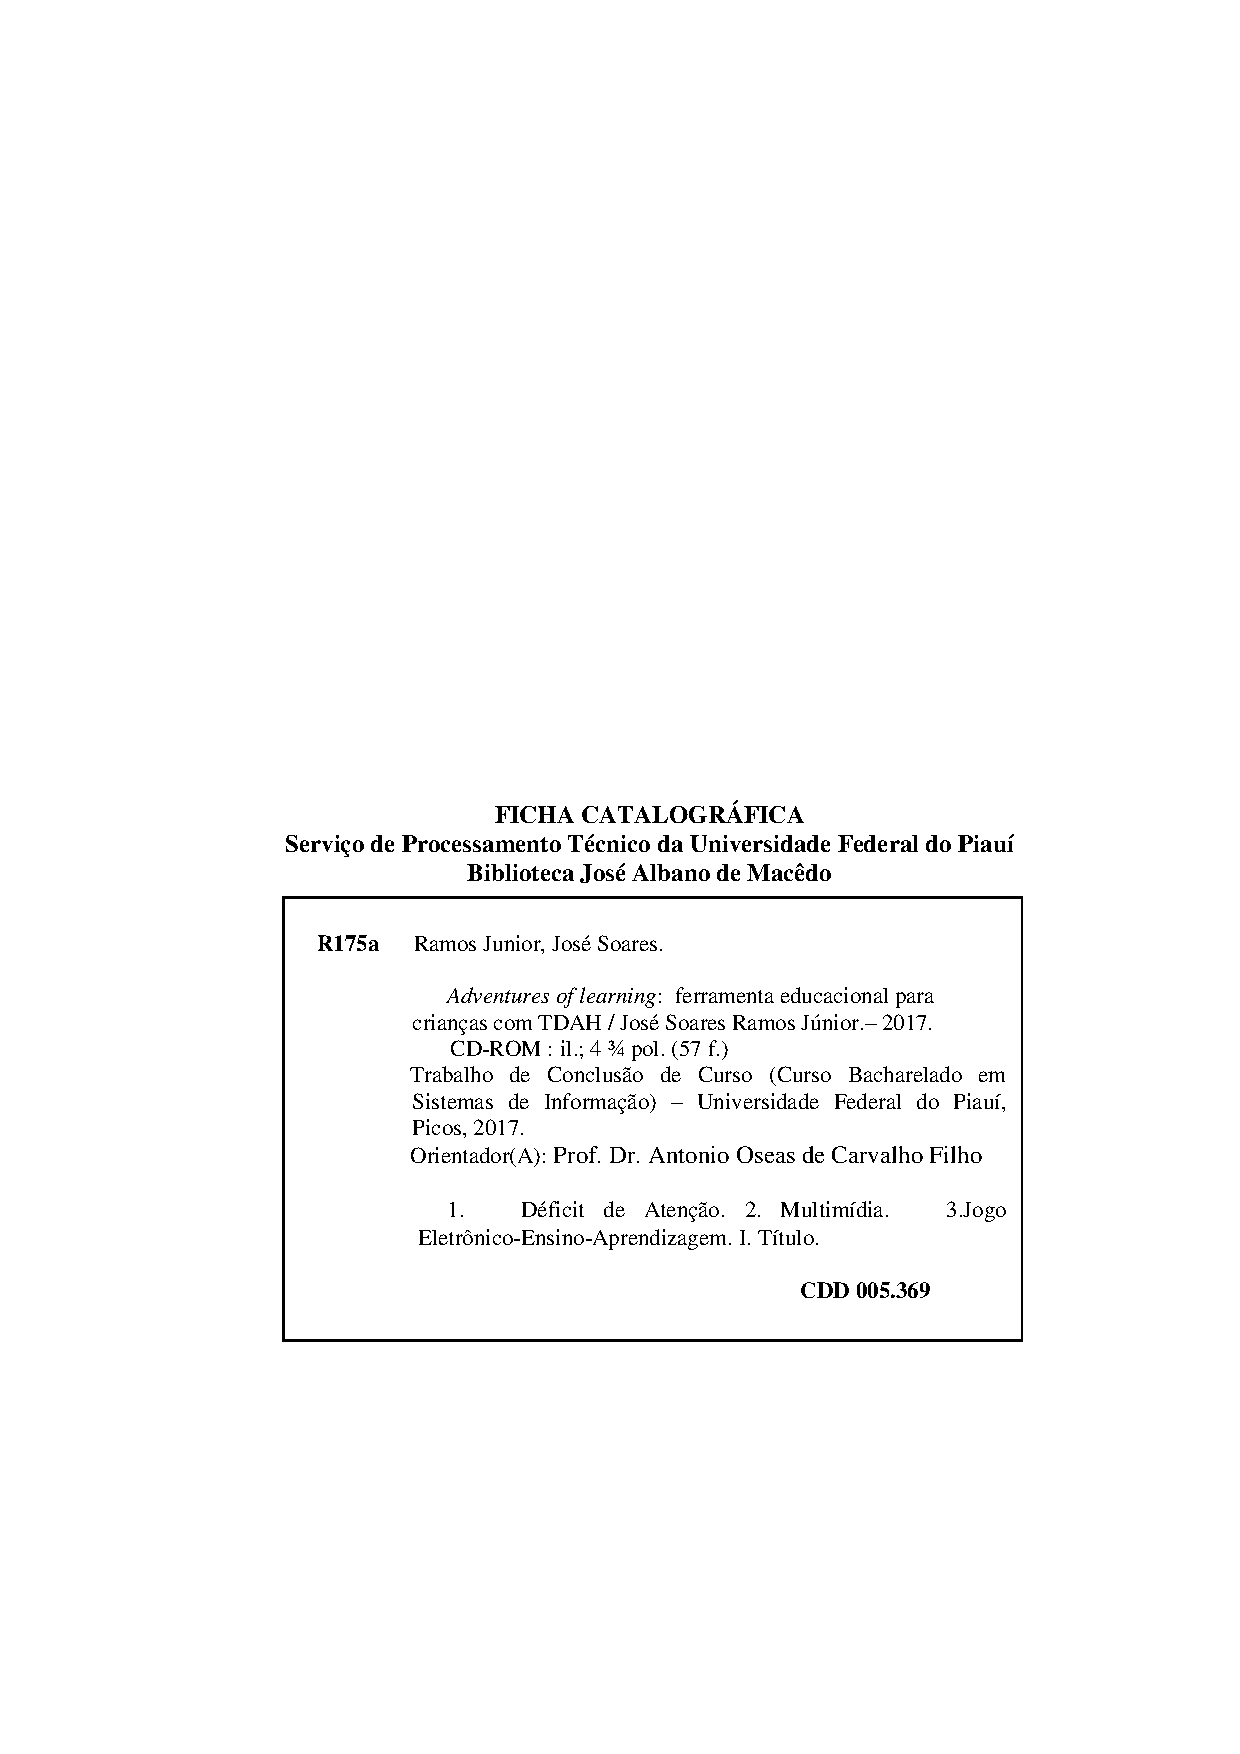
\includepdf{fig-ficha-catalografica.pdf}
\end{fichacatalografica}

\begin{folhadeaprovacao}
	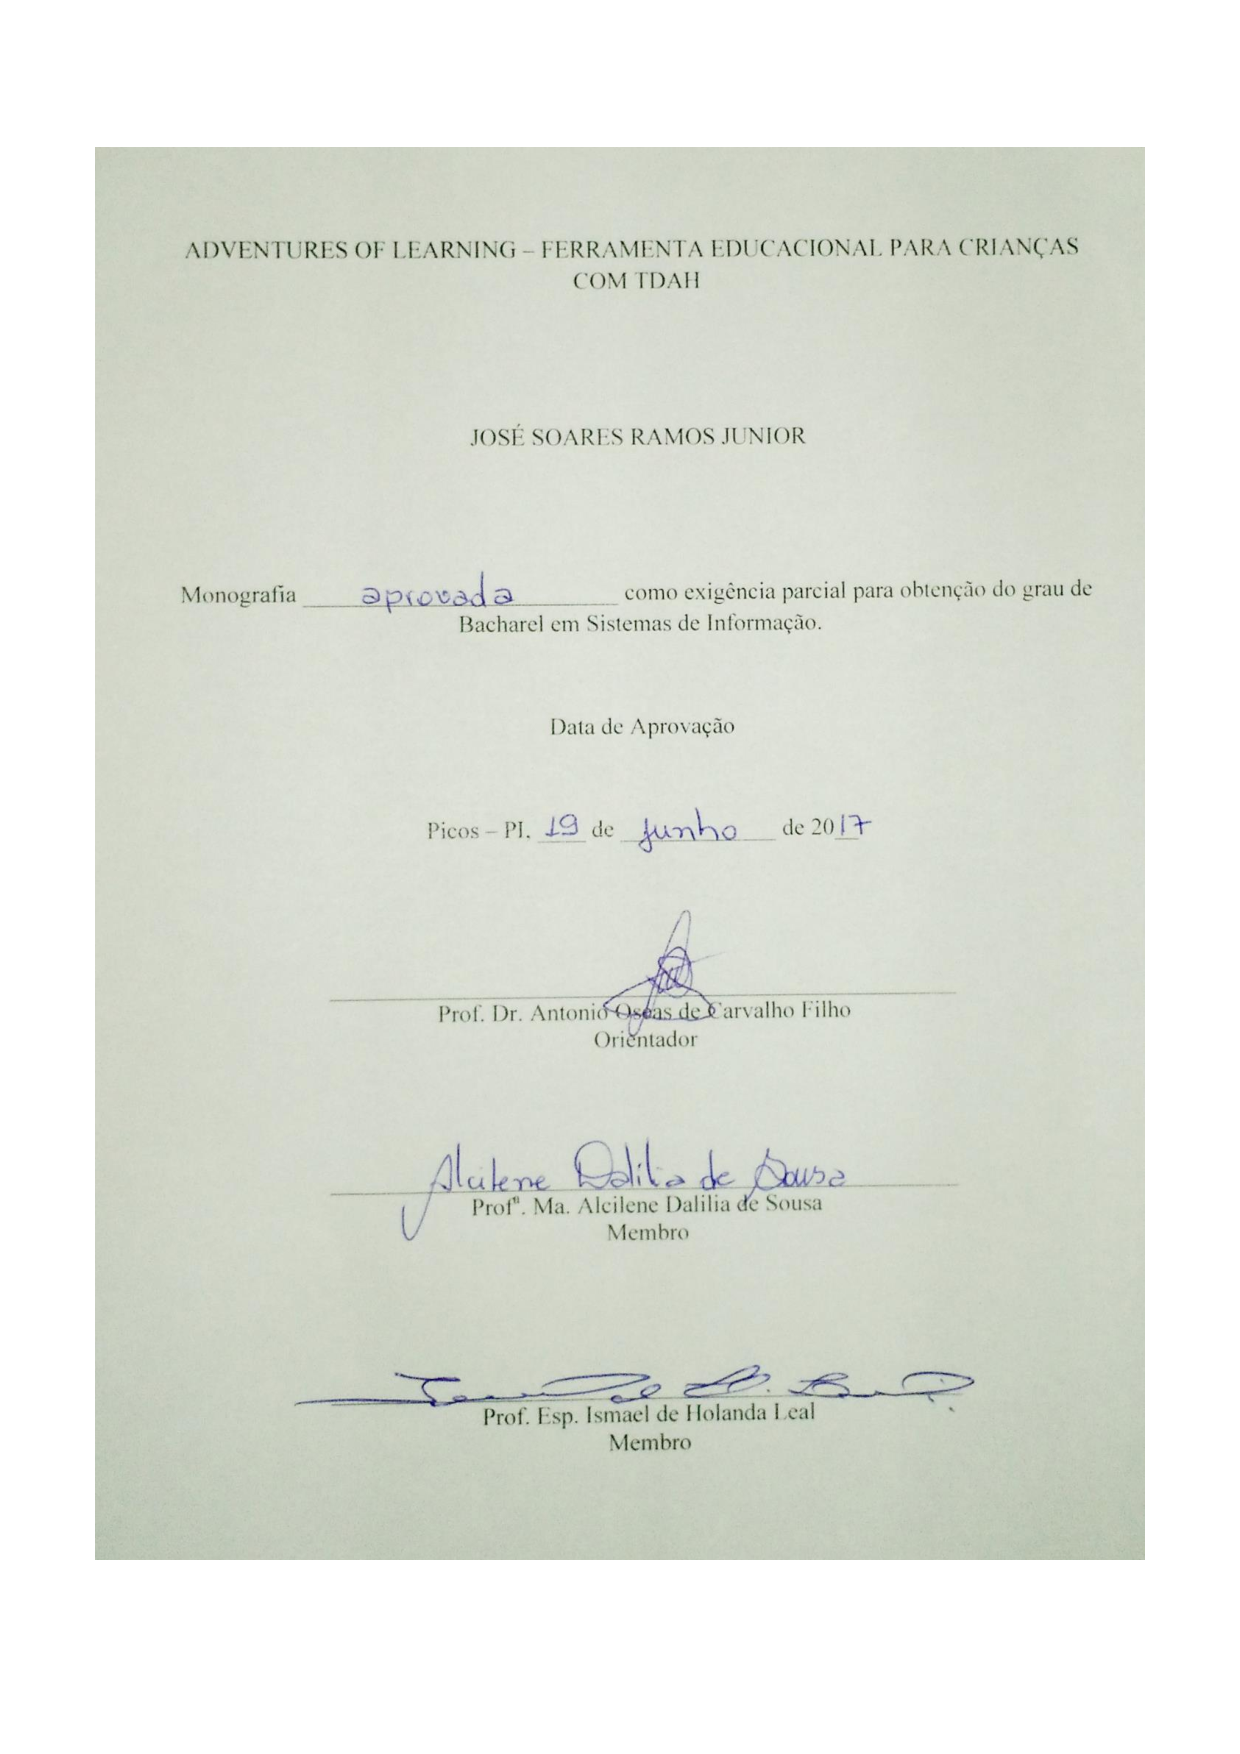
\includepdf{folha-de-aprovacao-escaneada}
\end{folhadeaprovacao}
% ---
% Agradecimentos
% ---
\begin{agradecimentos}
	No fim dessa jornada que começou no início de 2012, é meio difícil lembrar de todos aqueles que me ajudaram neste percurso, mais em especial agradeço a Deus pois sem ele nada seria possível. Agradeço a Universidade Federal do Piauí (UFPI), por me fornecer a oportunidade de cursar o curso que sempre sonhei em cursar. Deixo meus agradecimentos sinceros ao meu orientador Antonio Oseas, pela colaboração e força neste trabalho, ao professor Leonardo por ser um grande amigo, e a todos os demais professores que me ajudaram durante o curso. 
	Agradeço a uma pessoa especial que me levantou e meu deu forças em todos os momentos da minha, ela que além de ser minha mãe teve o papel de pai (Maria Edileusa), agradeço ao meu irmão Werlon por ser o pentelho da minha vida, ao meu avô (\textit{in memoriam}) que me mostrou como ser um homem de verdade, e a toda minha família que me forneceu força durante toda minha vida. Gostaria de agradecer minha namorada por me aguentar nesses últimos dias de estresse e a todos os meus grandes amigos que compartilharam momentos complicados e felizes, em especial ao Juliano, Laio, Josafá, Jaílson, Zé (José Roberto) e a todos os outros que não citei, preciso lembrar dos meus amigos servidores, seu Paulo, a tia da cantina pelo café de todos os dias. 
		
\end{agradecimentos}
% ---

% ---
% Epigrafe
% ---
\begin{epigrafe}
	\vspace*{\fill}
	\begin{flushright}
		\textit{Que os vossos esforços desafiem as impossibilidades,\\ 
				lembrai-vos de que as grandes coisas do homem foram \\
				conquistadas do que parecia impossível.\\
			Charles Chaplin}
	\end{flushright}
\end{epigrafe}
\pagebreak


% ---
% RESUMO
% ---

% resumo na língua vernácula (obrigatório)
\begin{resumo} %% AQUI COMEÇA A PÁGINA DE RESUMO
	A educação é um dos principais pilares para o avanço da sociedade, sejam estes em âmbito cientifico ou social. No processo educacional, educadores e educandos possuem o papel de enfrentarem juntos problemas que possam vir a surgir, para que assim o educando possa herdar o conhecimento que o educador deseja repassar. Um problema que afeta diversos alunos, que não discrimina idade, sexo, nível econômico ou qualquer outro fator recebe a denominação de Transtorno de Déficit de Atenção e Hiperatividade (TDAH), presente em quase todas as salas de aula de escolas, trazendo consigo problemas para o aprendizado do aluno através dos seus sintomas. Um dos principais problemas causados pelo TDAH ao aluno, é dificuldade na concentração em atividades repetitivas e que possam ser entediantes. A utilização de ferramentas multimídia para auxilio do processo de ensino, dentre essas ferramentas os jogos digitais, podem prender a atenção de portadores de TDAH, facilitando o processo de concentração, abrindo a mente dos seus usuários para novos conhecimentos. O presente trabalho tem por objetivo apresentar o desenvolvimento de uma ferramenta, jogo eletrônico, que auxilie o processo de ensino de alunos com TDAH. O projeto foi desenvolvido através de ferramentas tecnológicas que facilitam o processo de criação de jogos, dentre estas \textit{Unity}, UML, \textit{Photoshop}, C\#. Durante e após o desenvolvimento a ferramenta foi testada para encontrar erros a serem corrigidos, e comprovar a aplicabilidade dentro do contexto inserido.
 \vspace{\onelineskip}
    
 \noindent
 \textbf{Palavras-chaves}: Déficit de Atenção, Multimídia ,Jogo Eletrônico, Ensino, Aprendizagem.
\end{resumo} %AQUI TERMINA A PÁGINA DE RESUMO


\begin{resumo}[Abstract]
	
	Education is one of the main pillars for the advancement of society, whether these in the scientific or social sphere. In the educational process, educators and students have the role of facing problems that may arise, so that the learner can inherit the knowledge that the educator wishes to pass through. A problem that affects several students, who does not discriminate age, sex, economic level or any other factor is called Attention Deficit Hyperactivity Disorder (ADHD), Present in almost all of them the school classrooms, bringing with them problems for student learning through their symptoms. One of the main problems caused by ADHD to the student is difficulty concentrating on repetitive activities that can be tedious. The use of multimedia tools for the teaching process, among these digital tools, they can hold the attention of people with ADHD, facilitating the process of concentration, opening the minds of users to new knowledge. The present work aims to present the development of a tool, electronic game that helps in the process of teaching students with ADHD. The project was developed through technological tools that facilitate the process of creating games, among these Unity, UML, Photoshop, C\#. During and after development the tool was tested to find errors to be corrected, and prove the applicability within the inserted contexto.
	\vspace{\onelineskip}
	
	\noindent
	\textbf{Key-Words}: Attention Deficit, Multimedia, Electronic Game, Teaching, Learning.

\end{resumo}


% ---
% inserir lista de ilustrações
% ---

\listoffigures* %% o * indica que não será incluso no sumário
\cleardoublepage %% Pula página
% ---

% ---
% inserir lista de tabelas
% ---

\listoftables*
\cleardoublepage
% ---

% ---
% inserir lista de abreviaturas e siglas
% ---
\begin{siglas}
	\item[BADS] \textit{Behavioural Assessment of Disexecutive Syndrome}
	\item[IDE] \textit{Integrated Development Environment}
	\item[TDAH] Transtorno de Déficit de Atenção e Hiperatividade
	\item[TI] Tecnologia da Informação
	\item[UML] \textit{Unified Modeling Language}
\end{siglas}
% ---

% ---
% inserir lista de símbolos
% ---
\begin{simbolos}
  \item[\#] Simbolo cerquilha
  \item[\%] Sinal de porcentagem
\end{simbolos}
% ---

% ---
% inserir o sumario
% ---

\tableofcontents*

% ---

% ----------------------------------------------------------
% ELEMENTOS TEXTUAIS  (necessário para incluir número nas páginas)
% ----------------------------------------------------------
\textual


% ----------------------------------------------------------
% Introdução
% ----------------------------------------------------------
\chapter{Introdução} %% NOVO CAPÍTULO (REPARE QUE ELE AUTOMATICAMENTE JÁ COLOCA O NÚMERO DO CAPÍTULO E JÁ ADICIONA NO SUMÁRIO)

	A educação, desde os tempos mais remotos aos atuais, é algo a ser buscado pelo homem na tentativa de saciar a sede por conhecimento, para \citeonline{belluzzo2002}, o anseio pela busca do desconhecido de novas fronteiras e produção de novos conhecimentos sempre impulsionaram e continuam a projetar a sociedade em direção ao desenvolvimento. A aprendizagem é algo que está presente no dia a dia de cada pessoa desde o seu nascimento, um exemplo é que ao nascer a criança tem sua primeira lição, que é aprender a respirar. A forma como se assimila o conhecimento repassado, por professores, filósofos entre outras experiências, causam grande impacto na vida de qualquer ser vivo. Atualmente, a formação intelectual de crianças e adolescentes em ambientes escolares e em alguns outros locais, principalmente os que mantêm o perfil rígido, se ouve por parte dos professores ou outros participantes dessas instituições relatos de crianças com problemas em seu aprendizado.
	
	Nas escolas, ou em outros locais pelo mundo se tem casos de crianças com seu aprendizado prejudicado, seja por excesso de desatenção ou por não conseguirem se adequar no ambiente. Essa dificuldade é encontrada em vários alunos e de diversas idades, os que estão na idade escolar são alguns dos mais atingidos, por estes não terem uma mentalidade ainda bem desenvolvida. Alguns destes problemas podem estar atrelados diretamente aos distúrbios psicológicos, alguns são facilmente confundidos com os casos de “má criação”, um destes distúrbios é chamado de Déficit de Atenção e Hiperatividade ou TDAH. Segundo \citeonline{rhode&barbosa2000}, a tríade sintomatológica clássica da síndrome caracteriza-se por desatenção, hiperatividade e impulsividade. Esse é um dos transtornos com maior índice de portadores, e um dos mais estudados desde a sua descoberta.
		

	\begin{citacao} 
		“Crianças com Transtorno de Déficit de Atenção com Hiperatividade (TDAH) – caracterizado por níveis excessivos de desatenção, hiperatividade e impulsividade, em termos de desenvolvimento – são mais frequentemente identificadas e tratadas no ciclo inicial do ensino fundamental. Estudos realizados no mundo todo revelam uma taxa de prevalência de TDAH equivalente a 5,29\% – intervalo de confiança de 95\%: de 5,01 a 5,56 – de crianças e adolescentes”\cite{charach}
	\end{citacao}

	O TDAH possui algumas formas de tratamento que são atualmente utilizadas em seus portadores, as duas principais são a farmacológica que utiliza medicamentos, e a psicoterapia. Segundo o Guia Prático \citeonline{app}, a combinação de tratamentos (medicação e psicoterapia), apesar de não apresentar significância estatística, é apontada por pais e professores como significativa, especialmente no desempenho acadêmico e em alguns sintomas específicos das crianças com TDAH. Mesmo o portador do transtorno passando por tratamento, alguns dos portadores possui dificuldades em seu processo de aprendizado, sendo necessário uma outra abordagem para que estes não sofram de prejuízos. Professores em algumas ocasiões fazem uso de novas ferramentas com intuito de aumentar a taxa de atenção de seus alunos, essas ferramentas tem o poder de prender com maior facilidade o que se está sendo repassando no processo de ensino.
		
	Para \citeonline{marquesandsilva}
	
	\begin{citacao}	
		“A evolução da tecnologia associada à educação tem vindo a favorecer a emergência de um novo conceito – \textit{Edutainment} – que se caracteriza essencialmente pela necessidade de fusão dos termos educação e entretenimento. Este último, tem vindo a prosperar pelo explosivo desenvolvimento de produtos multimédia de carácter lúdico que se tem verificado nos últimos anos”
	\end{citacao}
	
	Alguns dos melhores materiais multimídia, como vídeos, jogos, música entre outros, pode-se inserir processos a fim de facilitar o ensino. Os jogos eletrônicos, podem ser vistos como um dos melhores materiais multimídia, hoje estes estão presentes no cotidiano de grande parte das crianças e adolescentes. Fazendo-se uso dos jogos eletrônicos como ferramentas facilitadoras de ensino, pode-se conseguir um grande aumento na taxa de aprendizagem. Os jogos no processo de ensino e aprendizagem são ferramentas capazes de auxiliar no processo educativo, desde que sejam planejados e trabalhados de uma forma crítica, que possibilite a aprendizagem de uma maneira significativa ao aprendiz \cite{pietruchinski}.

	\section{Objetivos}

		\subsection{Objetivo Geral}
		
			Desenvolver uma ferramenta educacional, um jogo eletrônico que possa proporcionar divertimento de forma que possa prender a atenção dos portadores de TDAH, e ao mesmo tempo auxiliar o processo de aprendizagem e ensino tornando-se fonte de conhecimento.
			
		\subsection{Objetivos Específicos}
			Visando alcançar o objetivo principal, se faz necessário cumprir com alguns objetivos específicos, entre eles:
			
			\begin{itemize}
				\item Analisar os problemas enfrentados por portadores de TDAH no processo de aprendizagem.
				
				\item Modelar um projeto com base nos problemas enfrentados por portadores de TDAH de forma que apresente divertimento e conhecimento.
				
				\item Desenvolver protótipo do projeto, utilizando-se de tecnologias com foco principal no desenvolvimento de jogos como \textit{Unity} 5 desenvolvida pela empresa \textit{Unity Technologies}.
				
				\item Avaliar a ferramenta com base em testes práticos, discutindo a sua performance com a análise nos resultados finais.
			\end{itemize}
			
		
	\section{Organização do Trabalho}
		O trabalho a ser apresentado é composto por 5 capítulos:
		\begin{itemize}
			
			\item Capítulo 2 - Apresenta algumas soluções e trabalhos de outros autores que possuem afinidade com o tema abordado, trazendo alguns pontos a serem explorados.
			
			\item Capítulo 3 - Apresenta-se informações sobre o Transtorno de Déficit de Atenção/Hiperatividade (TDAH), como causas, impactos, tratamentos, alem das tecnologias e ferramentas que foram essenciais para o desenvolvimento total de todo o trabalho.
			
			\item Capítulo 4 - E demostrada o processo de desenvolvimento da ferramenta desde de sua projeção a oque foi utilizado em sua construção e testes que serviram para se ter conclusões.
			
			\item Capítulo 5 - Se tem uma conclusão dos resultados do desenvolvimento do trabalho, assim como onde este deve ser melhorado e o que pode ser encorporado beneficiando a resolução do problema.
		\end{itemize}




\chapter{Trabalhos Relacionados}

	Devido a grandes avanços tecnológicos, a tecnologia da informação (TI) está sendo inserida em quase todos os campos de conhecimento, colaborando para um avanço mutuo. No campo da ciência educacional e da saúde, a utilização de ferramentas computacionais não é uma novidade, visto que se tem como exemplos o uso dessas para reabilitação cognitiva, avaliações	neuropsicológicas, atividades pedagógicas, entre outras que podem ser citadas.
	
	No tratamento do TDAH, é possível encontrar ferramentas desenvolvidas que possuem grande potencial, algumas ja estão sendo utilizadas. \citeonline{butnik2005neurofeedback} faz uso de um conjunto de jogos computacionais especiais e técnicas de \textit{Neurofeedback} para modular de forma consciente suas ondas cerebrais tendo como consequência uma mudança de comportamento.
	
	Uma ferramenta com intuito de colaborar no âmbito do diagnóstico do TDAH foi desenvolvida em forma de um jogo eletrônico, este foi criado com base em um módulo de captura cognitiva e denominado de Mapa Zoológico, que tem como autores \citeonline{andrade2004mapa}. O trabalho teve como objetivo auxiliar o processo de diagnóstico de disfunções executivas, com foco no TDAH, baseado na Bateria \textit{Behavioural Assessment of Disexecutive Syndrome} (BADS), utilizada para avaliação do comprometimento da função de planejamento em quadros disfunção executiva. 
	
	Um trabalho proposto por \citeonline{rizzo2009virtual}, na qual foi desenvolvido com tecnologia de realidade virtual um sistema de avaliação para crianças portadoras de TDAH, onde as crianças são avaliadas por meio de suas reações aos estímulos do sistema. A avaliação leva em conta o processo de processos de desatenção, hiperatividade, comportamento no ambiente.

% ---



% Capitulo de revisão de literatura
% ---
\chapter{Referencial Teórico}

	Nesta capítulo, serão apresentados, o Problema a ser abordado assim como as Tecnologias, Ferramentas que foram utilizadas para o desenvolvimento deste trabalho.

% --- Seção dentro do capítulo
\section{Prejuízo causado pelo Transtorno de Déficit de Atenção ao aprendizado}

	Na educação, algumas vezes são encontradas dificuldades que devem ser superadas pelos docentes e pelos discentes, em alguns dos problemas encontrados, a causa acaba por persistir durante todo o processo de ensino dos discentes, tornando ainda mais difícil o seu período de aprendizado. Alguns dos problemas enfrentados no processo de aprendizagem podem ter origem neurológica, o que amplia a necessidade de cuidados. Um dos transtornos comuns encontrados na maioria dos ambientes, e que causa grande impacto negativo na vida de alunos e professores, se denomina transtorno de déficit de atenção e hiperatividade (TDAH).

	\citeonline{mesquita2009} em seu trabalho, afirma que:

	\begin{citacao}
		“O TDAH é considerado pelo discurso médico um problema neurológico que aparece na infância, ocorrendo, pela primeira vez, antes de sete anos de idade, e que pode acompanhar a adolescência e a vida adulta de um indivíduo. Quanto à etiologia, acredita-se em origem genética (mesmo sendo as causas precisas do TDAH ainda desconhecidas), representada por alterações no funcionamento do lobo pré-frontal do cérebro: área responsável pelo controle da atenção, da memória e também pelo autocontrole, pela organização e pelo planejamento.”
	\end{citacao}

	Uma das principais características facilmente observadas nos portadores desse transtorno são os comportamentos exagerados, que também são responsáveis por dificuldades enfrentadas em escolas e em outros ambientes. Portadores de TDAH podem ser facilmente distinguidos, pois estes acabam por apresentar os sintomas clássicos que são, desatenção acentuada, inquietação elevada, baixo estímulo para fazer trabalhos repetitivos e que podem ser tediosos, dificuldade em seguir regras rigorosas ou manter um certo comportamento que o force a suprimir estímulos. Todos os sintomas podem não se manifestar no mesmo indivíduo, podendo apresentar variações do transtorno, assim pode-se ver que um indivíduo podem apresentar somente a hiperatividade ou o déficit de atenção acentuado.
	
	
	\citeonline{peixotoErodrigues}, afirmam que:
	\begin{citacao}
		“O \citeonline{dsmiv} subdivide o TDAH em três tipos: TDAH com predomínio de sintomas de desatenção; TDAH com predomínio de sintomas de hiperatividade/ impulsividade; TDAH combinado. No sexo feminino predominam os sintomas de desatenção que, juntamente com o tipo combinado, acarretam uma taxa mais elevada de prejuízo acadêmico.”
	\end{citacao}

	O efeito causado na vida escolar dos portadores de TDAH podem ser terríveis. Por si só o aprendizado na escola de disciplinas como Matemática, Português entre outras, através de métodos antigos de ensino, acaba-se tornando entediantes e de difícil compreensão para alguns, tornado um trabalho árduo, com dificuldades imensas, e quando se soma a os problemas externos se tem em mãos novos níveis de dificuldades a serem superadas, onde muitas vezes o educador pode não estar preparado para repassar o ensino adequado, como no caso dos portadores de TDAH.
	
	O TDAH é um problema que além de prejudicar a vida escolar de seus portadores, irá juntamente dificultar suas interações sociais do dia-a-dia. As dificuldades de interações sociais devem-se ao fato de seus sintomas exagerados geralmente causarem desconforto às pessoas próximas, ocorrendo um distanciamento por parte de amigos e familiares.
	
	Segundo \citeonline{smithandstrick} :
	\begin{citacao}
		“Muitos casos de TDAH não são percebidos até o início da escola – em cujo ponto os problemas parecem multiplicar-se em uma base diária. Os professores queixam-se de que a criança interrompe, não se senta quieta, não presta atenção, não termina seus trabalhos ou não escuta. Incapaz de planejar ou de aderir a um curso de ação, a criança logo começa a decair em seu desempenho escolar. Talvez ainda mais doloroso, a criança é deixada para trás também socialmente. As crianças com o transtorno têm dificuldade para aprender regras de jogos e são impacientes quanto ao revezamento. Com frequência, elas verbalizam impulsivamente qualquer coisa que lhes venha à mente, sem considerar o efeito de suas palavras. Os companheiros tendem a considerá-las rudes, intrometidas e insensíveis. Quando convites de aniversário são distribuídos e cartões de festas trocados, a criança com TDAH logo percebe o que os companheiros sentem a seu respeito. A rejeição social, juntamente com o baixo desempenho escolar, é uma boa receita para a perda da auto-estima. Muitas dessas crianças começam a ver a si mesmas como perdedoras em uma idade precoce.''
	\end{citacao}


\section{Jogos e Brincadeiras no Auxilio da Aprendizagem}

	Professores e educadores, em alguns casos quando se deparam com portadores de TDAH em sala de aula buscam soluções que possam beneficiar a aprendizagem destes alunos, para que assim estes consigam ter um desenvolvimento igual aos seus colegas de classe. Algumas soluções utilizadas para o auxílio de crianças com TDAH e outras que possuam problemas de aprendizagem, é a utilização do lúdico como forma de ensino, utilizando-se de jogos e brincadeiras para lhes apresentar conhecimento. Quando se utiliza o lúdico para o ensino se percebe algumas diferenças, isso se deve ao fato das crianças poderem se expressar de forma espontânea, tornando todo o processo mais simples, principalmente em crianças que possuem problemas como os portadores de TDAH.
	
	Segundo \citeonline{melo2011}:
	\begin{citacao}
		“Quando a criança envolve-se com o lúdico, ela tem a possibilidade de vencer medos, angústias, traumas e tudo que consiste a sua sensibilidade. É necessário que o brincar seja espontâneo e este deverá refletir a forma de pensar e sentir da criança, onde ela demostra sua história de vida”
	\end{citacao}
	
	Existem muitas possibilidades de jogos a serem utilizados como forma de auxilio no ensino, alguns são utilizados em tratamentos de crianças com distúrbios como o TDAH e Dislexia, o jogo da memória é um exemplo a ser utilizado, segundo \citeonline{cunha1997brincar} o jogo da memória estimula o pensamento, memorização, identificação de figuras, estabelecimento do conceito de igual e diferente e orientação espacial. Existem outros jogos a serem citados, cada um pode desenvolver uma parte em especifico.
	
	Para \citeonline{stroh2010tdah}:
	\begin{citacao}		
		“Existem algumas técnicas que são mais utilizadas durante o “tratamento” de um TDAH com o psicopedagogo, como: jogos de exercícios sensório-motores (amarelinha, bola de gude), combinações intelectuais (damas, xadrez, carta, memória, quebra-cabeça, etc.)”
	\end{citacao}
% --- Seção dentro do capítulo
\section{Tecnologias}

	Durante o desenvolvimento do projeto se fez necessário o uso de várias tecnologias, essas foram empregadas em conjunto, cada uma abordando uma função específica dentro do trabalho. A seguir tem-se a descrição das que foram utilizadas.

	\subsection{Levantamento de Requisitos}
		
	No processo de desenvolvimento de \textit{softwares}, o levantamento de requisitos ganha uma grande importância, isto se deve ao fato do mesmo permitir que se consiga desenvolver um trabalho com qualidade e que cumpra com o desejado. Por meio do levantamento de requisitos se consegue ter uma base de quanto irá custar, quanto tempo irá levar, e quais são as reais necessidades que este deve saciar, sem este levantamento, muitas vezes por mais qualificada que seja a equipe de desenvolvimento o \textit{software} acaba por não atender as necessidades essenciais, causando dor de cabeça com mais gasto de recursos e novos problemas. No levantamento de requisitos é levado em conta todas as atividades que serão desempenhadas pelo produto final, desde de as funcionalidades mais simples às mais complexas.
	
	Segundo \citeonline{wazlawick}:
	
	\begin{citacao}
		“O levantamento preliminar de requisitos tem por objetivo prover uma visão do todo, para poder definir o que é mais importante e depois dividir o todo em partes para especificar os detalhes. Nessa fase, o levantamento é rápido e genérico, sendo feito em extensão e não em profundidade. O analista deve entender a extensão do que o sistema deve fazer, mas sem entrar em detalhes.”
	\end{citacao}
	
	Em alguns casos encontra-se características diferenciadas, isto se deve ao fato de alguns tipos de \textit{softwares} como os de foco educativo, necessitarem de uma atenção a mais, principalmente por os problemas a serem solucionados por estes possuírem uma complexidade anormal .
	
	\subsection{Modelagem de Software com UML}
	
	Após o levantamento de requisitos, onde este deve demonstrar todas as características, necessidades e funcionalidades que deverão estar presentes no produto a ser desenvolvido, deve-se iniciar o processo de criação da documentação. Dentro da documentação\footnote{A documentação de software ou documentação do código fonte, é um texto escrito que acompanha o software e geralmente explica como utilizá-lo.} de software, estará presente a modelagem do sistema, onde pode-se utilizar \textit{Unified Modeling Language} (UML), com isto, é possível através de diversos diagramas obter uma visualização inicial de como deve funcionar o sistema e suas funcionalidades.
	
	Para \citeonline{guedes2009}:
	\begin{citacao} 
		“A modelagem de um software implica em criar modelos de software, mas o que é realmente um modelo de software? Um modelo de software captura uma visão de um sistema físico, é uma abstração do sistema com um certo propósito, como descrever aspectos estruturais ou comportamentais do software. Esse propósito determina o que deve ser incluído no modelo e o que é considerado irrelevante. Assim um modelo descreve completamente aqueles aspectos do sistema físico que são relevantes ao propósito do modelo, no nível apropriado de detalhe.”
	\end{citacao}
	
	O UML é composto por uma gama de diagramas, onde cada um possui sua função e característica, devido a essa variedade se tem em mãos uma ferramenta valiosa no gerenciamento e criação de \textit{softwares}, que, se bem utilizada pode acelerar o processo de desenvolvimento, e diminuir os erros que podem vir a ocorrer durante este processo.
	 
	\citeonline{guedes2009} ainda diz que:
	\begin{citacao}
		“Cada diagrama da UML analisa o sistema, ou parte dele, sob uma determinada óptica. É como se o sistema fosse modelado em camadas, sendo que alguns diagramas enfocam o sistema de forma mais geral, apresentando uma visão externa do sistema, como é o objetivo do Diagrama de Casos de Uso, enquanto outros oferecem uma visão de uma camada mais profunda do software, apresentando um enfoque mais técnico ou ainda visualizando apenas uma característica específica do sistema ou um determinado processo. A utilização de diversos diagramas permite que falhas sejam descobertas, diminuindo a possibilidade da ocorrência de erros futuros.”
	\end{citacao}
	
	Cada diagrama do UML permite que seja possível perceber uma nova perspectiva do sistema. Estes diagramas podem possibilitar a visualização do sistema na ótica do usuário através do diagrama de caso de uso, e pode fornecer ao desenvolvedor através do diagrama de classes uma direção a ser seguida no desenvolvimento do produto. Os diagramas podem ser comparados com os vários tipos de plantas de construção, pois, assim como um mestre de obras utiliza uma planta para construção de um edifício, o desenvolvedor utiliza os diagramas para desenvolvimento de uma aplicação.
	
		\subsubsection{Diagrama de caso de uso}
		
			Este diagrama tem por objetivo auxiliar o desenvolvedor a exibir as funcionalidades do sistema pelo ponto de vista do usuário. Este tipo de diagrama descreve cada funcionalidade, assim como, quem as desempenha no sistema, Pode-se visualizar na Figura \ref{fig:01} um exemplo de diagrama de caso de uso para melhor entendimento.
		
			\begin{figure} [hbt]
			\caption{Exemplo de diagrama de caso de uso.}
			\centering
			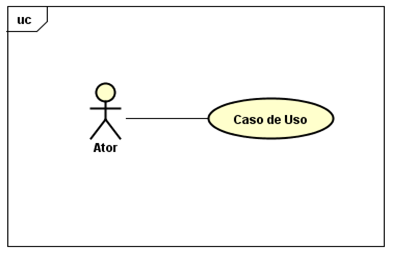
\includegraphics[width=0.7\linewidth]{Imagens/01}
			\legend{Fonte: O autor.}
			\label{fig:01}
			\end{figure}
		
		\subsubsection{Diagrama de classes}
			O diagrama de classes tem como objetivo fornecer uma visualização do sistema ao desenvolvedor, exibindo um conjunto de classes com seus atributos, métodos e relacionamentos. Esse tipo de documentação é geralmente encontrado em projetos que sejam orientados a objetos\footnote{A orientação a objetos é um paradigma de análise, projeto e programação de sistemas de software baseado na composição e interação entre diversas unidades de software chamadas de objetos}, onde é possível a estruturação do sistema por meio de classes que devem representar os objetos, assim como suas sequências e estados. Na Figura \ref{fig:02}, é possível visualizar um exemplo de diagrama de classes, com a visualização de classes ativas no sistema.	
			\begin{figure}[H]
				\caption{Exemplo de diagrama de classes.}
				\centering
				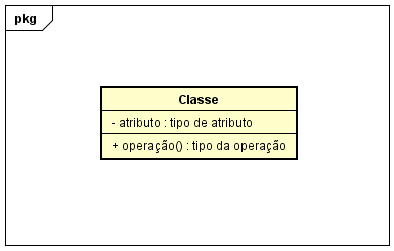
\includegraphics[width=0.5\linewidth]{Imagens/02}
				\legend{Fonte: O autor.}
				\label{fig:02}
			\end{figure}
		
		Apesar do UML possuir muitos outros tipos de diagramas, algumas vezes estes podem acabar por complicar o planejamento e a execução de um projeto. A utilização dos diagramas de caso de uso e classes em pequenos projetos podem suprir as necessidades, desde de que se tenha uma visão do todo e que seja analisado os fatos.
		
		
	\subsection{Motores Gráficos (\textit{Game} \textit{Engine})}
	
		Os motores gráficos, atualmente são os maiores colaboradores no desenvolvimento de aplicações gráficas, como jogos virtuais ou outras aplicações do gênero gráfico. O motor gráfico ou \textit{game} \textit{engine} como são chamados, na realidade são conjuntos de bibliotecas que auxiliam o desenvolvimento de aplicações, ou seja, seu objetivo é simplificar a codificação para evitar que tudo seja feito a partir do zero. Um dos maiores trunfos dessas ferramentas é a facilidade oferecida para modelar objetos 2D e 3D, podendo estes serem acompanhados de animações e sons.
		
		Para \citeonline{clua2005desenvolvimento}:
		\begin{citacao}
			“Dentro da área de jogos, um engine se encarregará por entender-se com o hardware gráfico, irá controlar os modelos para serem renderizados, tratará das entradas de dados do jogador, tratará de todo o processamento de baixo nível e outras coisas que o desenvolvedor de jogos normalmente não deseja fazer ou não tem tempo para se preocupar. Existem inúmeras definições para um engine.”
		\end{citacao}
	
	\subsection{\textit{Game} \textit{Design}}
		
		O \textit{Game} \textit{Design} possui um dos papéis fundamentais no desenvolvimento de jogos, pois estes são encarregados de pensar como deve ocorrer as interações dentro dos jogos, ou seja, suas temáticas, funcionalidades, padrões, enredos e toda as suas dinâmicas.
		
		\citeonline{clua2005desenvolvimento} conceituam o \textit{game} \textit{design}:
		\begin{citacao}
			“Entende-se por \textit{game design} a conceituação artística do jogo. Hoje em dia, dada a complexidade das histórias e dos cenários elaborados é importante que esta parte do documento seja escrita por um artista. Dentro deste item deverão ser expostos quais as principais características dos cenários, esboços de personagens, descrição das texturas fundamentais, mapas e descrições das fases (também denominado de level design).”
		\end{citacao}
		
		Conforme foi dito por \citeonline{clua2005desenvolvimento}, o papel do \textit{game} \textit{design} é de grande importância dentro do projeto, mais este não é atrelado somente a parte gráfica, algumas outras funções são de sua responsabilidade, onde estas têm grande importância dentro do jogo.
		
		\citeonline{rouse2010game} afirma que:
		\begin{citacao}
			“O \textit{game design} determina quais escolhas o jogador será capaz de fazer no mundo do jogo e que ramificações estas escolhas terão no restante do jogo. O \textit{game design} determina qual o critério de ganho ou perda o jogo deverá incluir, como o usuário será capaz de controlar o jogo e que informações o jogo comunicará a ele, e isto estabelece o quão difícil o jogo será. Resumidamente, o \textit{game design} determina todos os detalhes de como a jogabilidade funcionará.”
			
		\end{citacao}
	\subsection{Linguagem C\# (C sharp)}
		O C\# é uma linguagem de programação, desenvolvida pela empresa \textit{Microsoft} em 2001. Essa linguagem se mostra extremamente versátil, que tem como caracteristicas ser uma linguagem interpretada\footnote{Linguagem interpretada é uma linguagem de programação em que o código fonte nessa linguagem é executado por um programa de computador chamado interpretador, que em seguida é executado pelo sistema operacional ou processador.} e fortemente tipada\footnote{Linguagem tipada, ou linguagem tipificada, é uma linguagem de programação que usa variáveis com tipos específicos.}, além de ser multi-paradigma abordando os paradigmas de programação orientado a objetos, imperativa, funcional, declarativa e genérica.
		
		\citeonline{deitel2002} cita alguns pontos a serem observados:
		\begin{citacao}
			“A linguagem de programação C\#, desenvolvida pela Microsoft por uma equipe liderada por Anders Hejlsber e Scott Wiltamuth, foi projetada especificamente para a plataforma .NET como linguagem que permite aos programadores migrarem facilmente para o .NET. Essa migração é facilitada graças ao fato de que o C\# tem raízes em C, C++ e Java, adaptando os melhores recursos de cada linguagem e acrescentando novas capacidade próprias. Como o C\# foi construído com base em linguagens amplamente usadas e bem desenvolvidas, os programadores acharão seu aprendizado fácil e agradável.”
		\end{citacao}
	
	\section{Ferramentas}
	
		A utilização de ferramentas pelo ser humano é algo natural que vem ocorrendo desde a pré-história, onde os seres humanos primitivos faziam uso de ferramentas construídas principalmente a partir de lascas de pedra sendo estas praticamente indispensáveis para sobrevivência. O principal motivo para utilização de ferramentas pelo ser humano em suas atividades se deve ao fato das contribuições que estas fornecem, como acelerar os processos de preparação e criação de produtos, aumento de qualidade e inovações. No desenvolvimento de \textit{softwares} e afins, diversas ferramentas que podem contribuir para o desenvolvimento de um trabalho de qualidade superior com tempo ágil. A seguir pode-se visualizar a descrição de ferramentas utilizadas no desenvolvimento deste trabalho.
		
		\subsection{Astah Professional}
			
			O Astah Professional, é uma ferramenta de modelagem UML muito utilizada para o desenvolvimento de diagramas e afins, por desenvolvedores e estudantes. O Astah é uma das boas opções no mercado entre as ferramentas de modelagens, isto se deve ao fato de sua licença ser do tipo \textit{freeware}\footnote{Software gratuito ou freeware é qualquer programa de computador cuja utilização não implica no pagamento de licenças de uso ou royalties.}, ou seja, concede uma licença para utilização de forma gratuita apesar de não ser \textit{open-source} (código aberto), se mostrando bastante poderosa no que se propõe a fazer.
			
			Segundo \citeonline{ribeiro2012}:     	
				\begin{citacao}
				“O \textit{Astah} é uma ferramenta que visa auxiliar o processo de modelagem de um sistema, é um editor de diagramas UML que incorpora outros recursos de acordo com a distribuição utilizada. É sucessora do JUDE (\textit{Java and UML Developers Environment} – Ambiente para Desenvolvedores UML e Java), ferramenta que foi descontinuada em 2010. Assim como o JUDE, esta ferramenta possui versões \textit{CommUnity} e \textit{Professional}.”
				\end{citacao}
			
			Para utilização da ferramenta não é necessário empenhar um grande esforço, seu \textit{layout} apresenta as funcionalidades de forma simples. Com o \textit{astah} se pode modelar diagramas complexos em curtos períodos de tempo, de forma simples podendo acelerar o processo de desenvolvimento. 
		
		\subsection{Unity 5}
			
			O \textit{Unity} 5 é uma ferramenta de grandes recursos desenvolvida pela empresa de tecnologia \textit{Unity Technologies}, com sua primeira versão lançada em 2005, essa ferramenta foi criada com o objetivo de facilitar o desenvolvimento de \textit{games} e conteúdos interativos 2D/3D. O \textit{Unity} 5 se destaca no cenário de desenvolvimento de jogos, fornecendo a possibilidade de criação de \textit{games} multiplataforma com sua poderosa ferramenta de forma simples, isso é possível graças a integração do motor gráfico e IDE\footnote{ Integrated Development Environment ou Ambiente de Desenvolvimento Integrado, é um programa de computador que reúne características e ferramentas de apoio ao desenvolvimento de software com o objetivo de agilizar este processo}, que apresenta ao desenvolvedor uma forma intuitiva de criação, tornando possível que pessoas sem formação ou experiência na área de criação de jogos criarem seus próprios projetos.
			
			Segundo a \citeonline{unity2017a}:
			\begin{citacao}
				“Você pode criar qualquer jogo em 2D ou 3D com \textit{Unity}. Pode fazê-lo com facilidade, pode torná-lo altamente otimizado e bonito, e pode implantá-lo com um só clique para mais plataformas que o número dos dedos de suas mãos e pés. Além disso, pode usar os serviços integrados de \textit{Unity} para acelerar seu processo de desenvolvimento, otimizar seu jogo, conectar-se com um público, e triunfar.”
			\end{citacao}
			
				A flexibilidade oferecida pelo \textit{Unity} 5 é de extrema utilidade aos desenvolvedores que desejam atingir grandes públicos com suas criações. A ferramenta permite a exportação de seus projetos para diversas plataformas, sem a necessidade de alterações de códigos e configurações.
				
			A \citeonline{unity2017b} ainda diz que:
			\begin{citacao}
				“Existem muitas plataformas que permitem a implantação com o mecanismo de jogos \textit{Unity}, e esse número está sempre aumentando. Crie seu conteúdo uma vez e implante-o com um clique nas principais plataformas para dispositivos móveis, VR, \textit{desktop}, console, e plataformas TV além da Web.”
			\end{citacao}
		
	\subsection{Adobe Photoshop}
	
		O \textit{Photoshop} é uma ferramenta de desenvolvimento gráfico amplamente utilizado em diversas áreas, o software é desenvolvido e licenciado pela empresa Adobe \textit{Systems}. O \textit{software} está disponível para ser utilizado em alguns sistemas, principalmente aos pertencentes às empresas \textit{Microsoft} a qual desenvolve os sistemas \textit{Windows}, e a \textit{Apple} responsável pelos computadores MAC com seus sistemas operacionais MAC OS. A ferramenta permite que seja possível criar artes gráficas com facilidade e qualidade, dependendo somente da criatividade do usuário.
		
		Segundo \citeonline{da2017desenvolvimento}:
		\begin{citacao}
			“O programa é composto por uma infinidade de recursos, que são utilizados para o melhoramento de imagens, extração de detalhes, suavização de altas frequências e pinturas digitais. Este \textit{software} trabalha com a metodologia de camadas, onde é possível editar a imagem dividida em partes.	O editor é completo, porém, exige um treinamento para melhor aproveitamento dos recursos oferecidos pelo \textit{software}. A empresa criadora do programa também oferece certificação para os interessados em comprovar seus conhecimentos com a ferramenta. ”
		\end{citacao}		
			
			
% ---	
\chapter{Metodologia}
	O processo de criação do jogo \textit{Adventures Of Learning} (Aventuras do Aprender) foi dividido em três fases, onde cada uma tem sua respectiva função e responsabilidade: análise de requisitos, modelagem de dados e a construção do jogo. Neste capítulo será abordado todas as fases citadas.
	
	\section{Análise de Requisitos}
	
		O ponto inicial para o desenvolvimento de \textit{softwares} é análise de requisitos, os jogos não são exceção, esse é o ponto de partida para o início do projeto. Por meio dessa análise é exposto o que deve ser implementado dentro do projeto. Quando a análise de requisitos é efetuada corretamente e com conformidade, obtém-se uma aceleração no desenvolvimento, isso se deve ao fato de poder focar o poder de trabalho nas áreas que necessitam de atenção especial dentro do projeto. Uma parte crucial que não deve ser deixado de lado é a análise do conteúdo pedagógico, visto que em \textit{softwares} educacionais esta é uma parte fundamental e de grande importância, onde se deve tomar cuidado ao inseri-los e explorá-los.
		 
		Nessa etapa foram decididos como deve funcionar as mecânicas do jogo, realizando uma análise e pesquisa, optou-se por uma fusão de jogos físicos em forma eletrônica com jogos clássicos eletrônicos que seguem o estilo plataforma\footnote{Jogo eletrônico de plataforma é o nome dado a um gênero de jogos eletrônicos em que o jogador corre e pula entre plataformas e obstáculos, enfrentando inimigos e coletando objetos bônus.}. Um dos recursos a ser utilizado é o jogo da memória, este foi escolhido pois estimula a concentração e o processo de memorização, sendo um dos materiais comprovadamente efetivos no auxílio do ensino.
		
		
		\citeonline{tavares2008apoio}, fala um pouco sobre esses materiais:
		\begin{citacao}
			“O que se comprovou  foi a existência de materiais de fácil acesso, como revistas dedicadas ao público infanto-juvenil, à venda em bancas de jornal, que oferecem atividades que podem ser perfeitamente  adaptadas às tarefas escolares como recursos favoráveis ao trabalho com as dificuldades citadas; Dislexia e TDAH, como por exemplo: “Jogos de memória”, “Palavras cruzadas”, “ Encontre os erros” e outros sugeridos nos Anexos I e II.” 
		\end{citacao}
		
		Nesta etapa ficou definido quais os atores presentes no jogo, e quais seriam suas respectivas ações dentro do mesmo. No diagrama de casos de usos, se representa o \textit{player} (usuário) como um Ator, e os inimigos como outro Ator. Como dito, o jogo possui dois Atores que são expostos no diagrama de casos de uso, onde suas principais funções são definidas.
	
		\subsection{Jogador (\textit{Player})}
		
			\begin{itemize}
				\item Informações – Durante a imersão no jogo, serão expostas informações que possam ser assimiladas por parte do usuário, colaborando no aprendizado na educação básica da leitura, escrita e matemática.
				\item Superar Desafios – Durante o jogo, o usuário será exposto a desafios a qual devem ser superados pelo \textit{player}. Os desafios são postos no caminho do usuário para que dificulte o caminho a ser percorrido, e para que o mesmo possa adquirir informações que no decorrer do jogo será de grande utilidade.
				\item Superar inimigos – Ao decorrer do jogo os inimigos irão aparecer nas fases, estes são encarregados de dificultar o avanço de fase do usuário os infligindo dano. Os inimigos com o poder de infligir dano ao usuário, podem zerar a vida\footnote{Representa a vida do personagem no jogo}, e quando isto ocorrer haverá um aviso de \textit{game over} após um tempo retornando ao menu inicial, assim sendo o usuário deverá encontrar uma maneira de passar pelos inimigos sem que estes serem sua vida.
				\item Avançar de fase – O objetivo principal do usuário no jogo é o avanço de fase. Para ser possível o avanço de fase o usuário deve superar todos os obstáculos e inimigos chegando ao seu ponto final.
				\item Desafios extras – Ao chegar no ponto final da fase o \textit{player} irá se depara com um desafio extra a qual ele deve completar para iniciar a próxima fase. Esses desafios podem ser jogos simples como o jogo da memória que é o primeiro e segundo desafio.
			\end{itemize}
		
		\subsection{Inimigo}
			\begin{itemize}
				\item Destruir \textit{player} – O único objetivo do inimigo no jogo e reduzir a “vida” do \textit{player} até que este chegue a zero, assim “destruindo” o mesmo ocorrendo logo em seguida a tela de \textit{game over}.
			\end{itemize}
		
		\subsection{Diagrama de Caso de Uso do \textit{Adventures Of Learning}}
		
			No diagrama de caso de uso (Figura \ref{fig:03}), são definidas e exibidas a funções que podem ser efetuadas por cada ator, na qual representam respectivamente o usuário e inimigos dentro do jogo.
			
			\begin{figure}[H]
				\caption{Diagrama de Caso de Uso do \textit{Adventures os Learning}.}
				\centering
				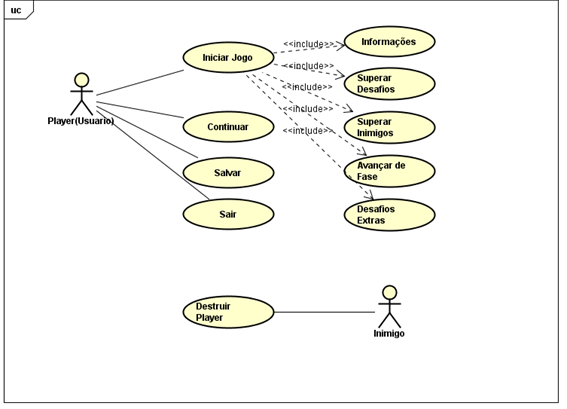
\includegraphics[width=0.7\linewidth]{Imagens/03}
				\legend{Fonte: O autor.}
				\label{fig:03}
			\end{figure}
		
		\subsection{Diagrama de Classe do \textit{Adventures Of Learning}}
			
			O diagrama de classes (Figura \ref{fig:04}) define e estrutura o projeto, facilitando a construção do mesmo. Neste é possível visualizar as funções e atributos pertencentes a cada objeto, e como estes devem estar dispostos.
			
			\begin{figure}[H]
				\caption{Diagrama de Caso de Classes do \textit{Adventures os Learning}}
				\centering				
				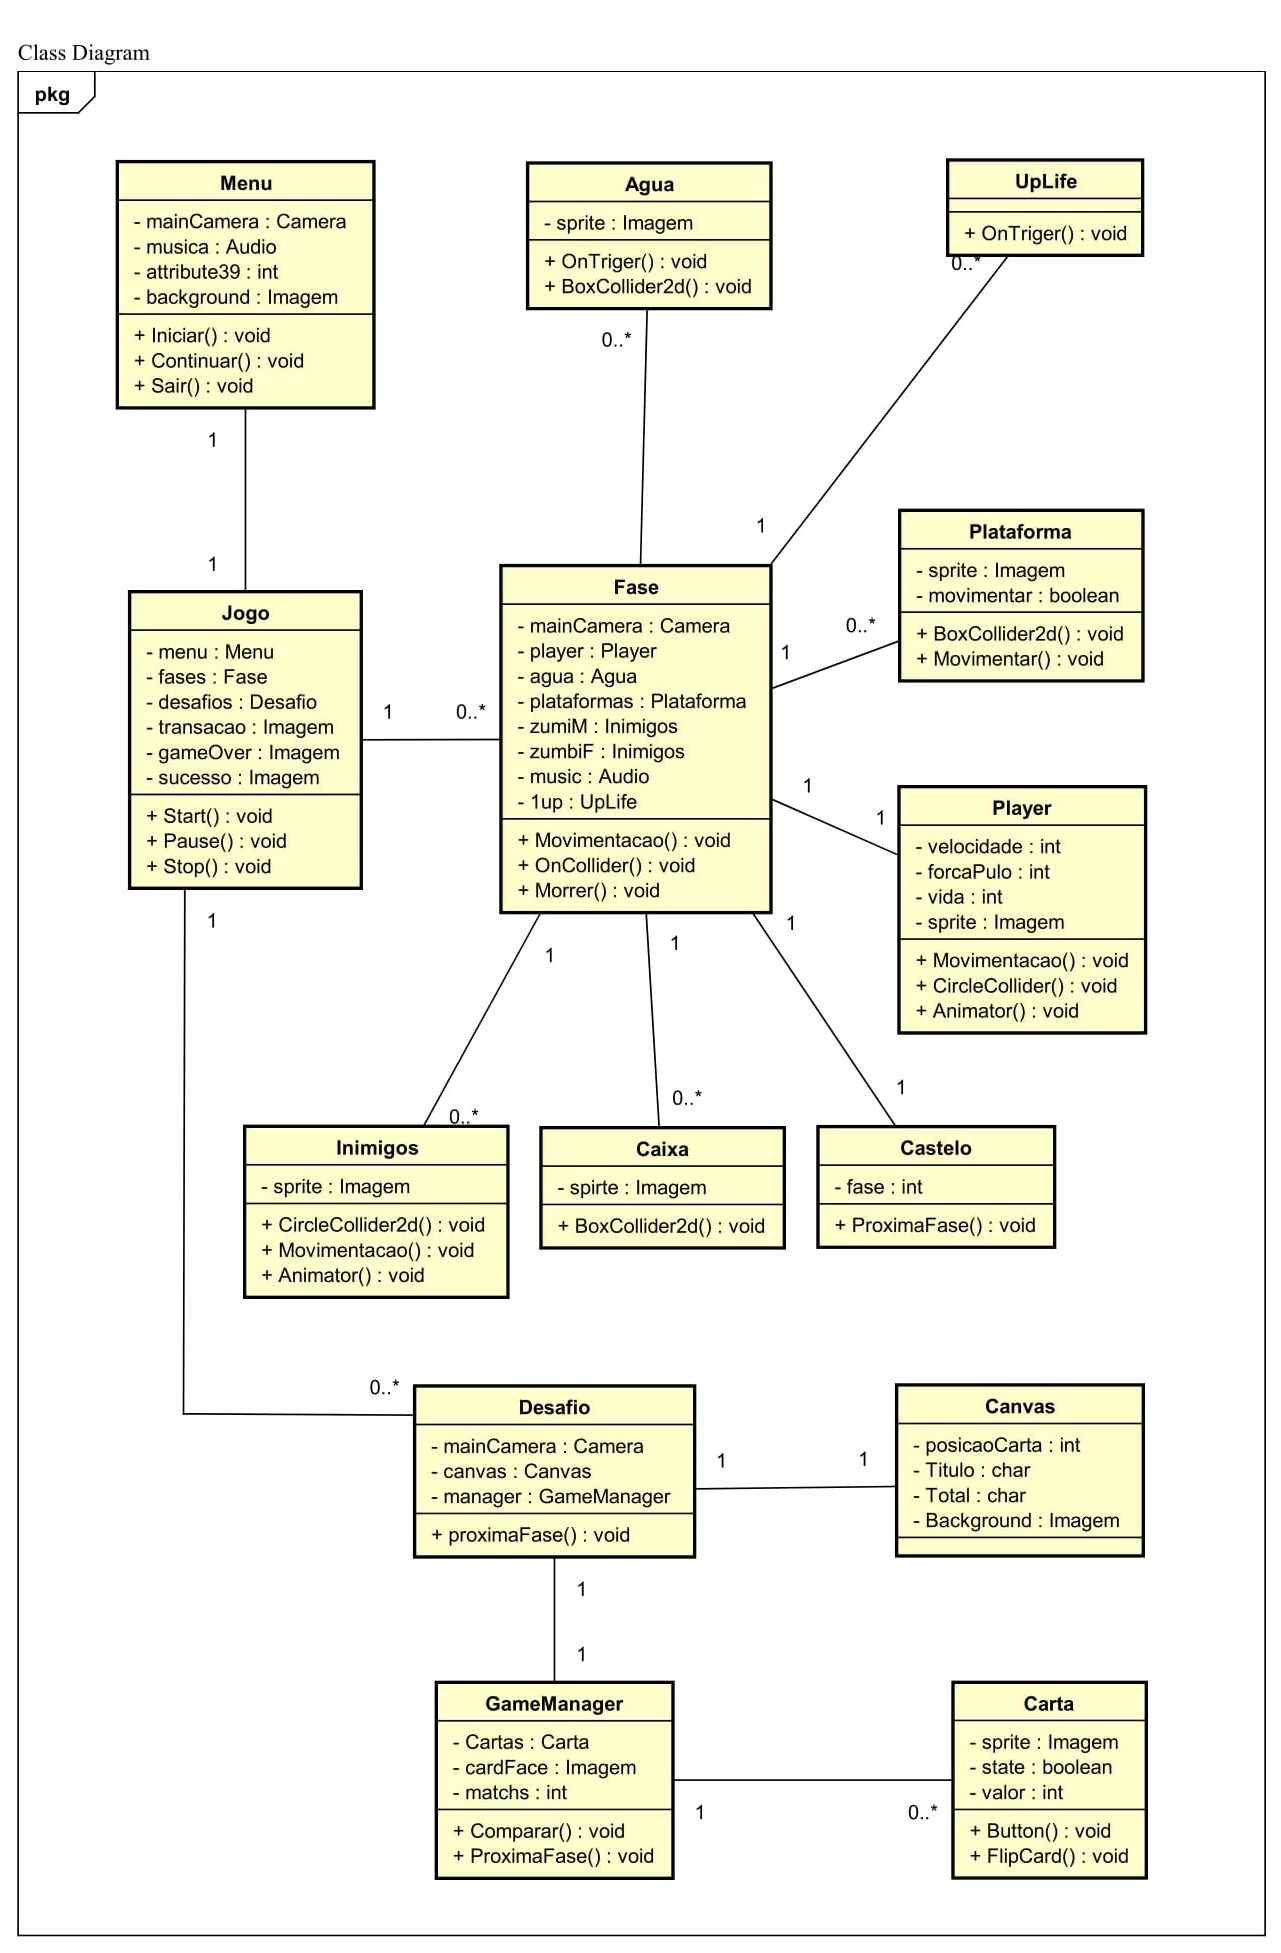
\includegraphics[width=1\linewidth]{Imagens/04}	
				\legend{Fonte: O autor.}			
				\label{fig:04}
			\end{figure}
			
		
	\section{Desenvolvimento  do Jogo}
		Nesta sessão são abordados todos os aspectos referentes à construção do jogo, detalhando os processos que ocorreram em seu desenvolvimento.
			
		\subsection{Interface Gráfica}
			A interface gráfica (Figura \ref{fig:05}) é um dos principais componentes dos jogos, visto que essa é a responsável pela representação e interação de todos os elementos de forma que se possa visualizá-los. É de suma importância que a interface seja intuitiva e de fácil entendimento, tornando o uso do software agradável aos olhos do usuário, isso possibilita que o jogador se concentre totalmente no que é proposto pelo jogo. 
			\begin{figure}[H]
				\caption{Menu inicial do jogo \textit{Adventures Of Learning}}
				\centering
				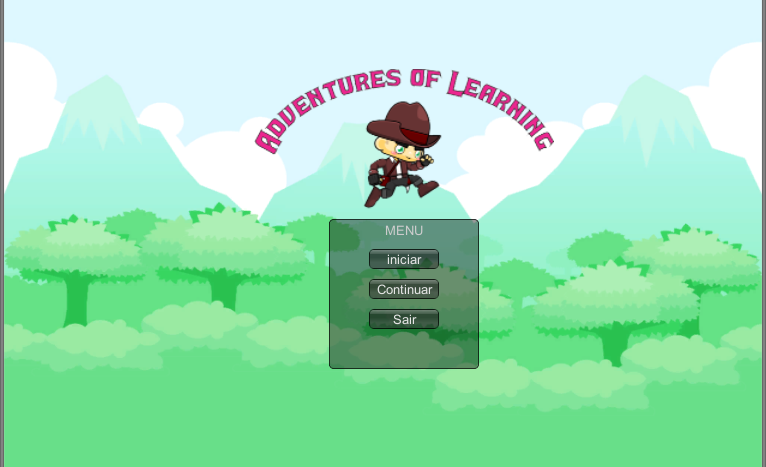
\includegraphics[width=0.7\linewidth]{Imagens/05}
				\legend{Fonte: O autor.}
				\label{fig:05}
			\end{figure}				
				
		\subsection{Modelagem do Jogo}
		
			A Modelagem do Jogo é parte em que se foca na criação dos elementos gráficos que estão presentes dentro do mesmo, como as formas geométricas dos cenários, personagens e objetos. A modelagem pode ser dividida em duas partes distintas, isso se deve ao fato de existirem dois tipos de objetos geométricos, sendo os objetos estáticos que não possuem atividade, que devem permanecer imóveis dentro do jogo, e os objetos dinâmicos onde estes possuem algum tipo de atividade, ou movimentação durante a execução do jogo, um exemplo de objeto dinâmico é o próprio personagem, já que esse pode se movimentar pelo cenário, e objetos estáticos plataformas que não se movem.
			
			A maior parte dos objetos que caracterizam um jogo estão presentes no cenário, pois o mesmo é o principal responsável por receber todos os objetos que fazem parte do ambiente. Na criação e desenvolvimento de jogos, se inicia o projeto com a modelagem de um cenário, onde se define cores, texturas e estilos.  
				
		\subsection{Funcionalidades do Unity 3D Utilizadas}
			O \textit{Unity} possui diversas funcionalidades que auxiliam o desenvolvimento de jogos. Neste tópico será explorado as funcionalidade que foram utilizadas no desenvolvimento deste projeto.
			
			\subsubsection{Project}
				O \textit{project} é a funcionalidade básica responsável por reunir e organizar os elementos que fazem parte do projeto. Nesta funcionalidade o desenvolvedor pode organizar da forma que desejar todos os arquivos referentes ao seu projeto, podendo adicionar e deletar arquivos e componentes da forma que se desejar. Para fins de organização se faz interessante montar uma forma hierárquica que facilite a distribuição e o manuseio de arquivos que fazem parte do projeto, isto traz agilidade e facilidade quando se procura um determinado objeto. O diretório \textit{Assets} possui outros diretórios que são responsáveis por armazenar um determinado tipo de arquivo do projeto, um exemplo seria diretório \textit{scripts} responsável por armazenar os \textit{scripts} utilizados no projeto.  
				
				
			\subsubsection{Scripts}
				\textit{Script} é um arquivo que contém alguns códigos, escritos em uma linguagem de programação, dentro deste são definido todas as instruções, regras e possibilidades que podem ocorrer. Todos os componentes dinâmicos pertencentes ao \textit{game} são controlados por um \textit{script} que define o comportamento que este deverá possuir dentro do projeto, desde a movimentação do \textit{player} as regras que definem o final do \textit{game}. A duas ferramentas que podem ser utilizadas no \textit{Unity} para criação dos \textit{scripts}, sendo estas duas IDE’s de codificação, \textit{Microsoft Visual Studio} e o \textit{Mono Develop} a utilizada neste projeto foi a IDE \textit{Microsoft Visual Studio}.
				Todas as capacidades que o \textit{player} pode desencadear dentro do jogo é controlada por um \textit{script} denominado “\textit{Player}”, onde estão escritos os métodos responsáveis por lhe fornecer as opções de andar, pular, cair e controlar suas animações e sons a serem executados.
				
			\subsubsection{Sprite}
				\textit{Sprite} (Figura \ref{fig:07}) é um objeto criado via ferramenta gráfica como \textit{Corel Draw} e \textit{Photoshop} com o intuito de representar de forma gráfica os objetos dentro do jogo, como \textit{player}, fundo, árvore, plataforma e todos os objetos que são possíveis de se visualizar dentro do jogo. Basicamente uma sprite adota o formato png\footnote{ formato de dados utilizado para imagens, que surgiu em 1996 como substituto para o formato \textit{Portable Network Graphics} (PNG), também conhecido como PNG's \textit{Not GIF}} devido ao pouco espaço que ocupa e a possibilidade de salvar os arquivos sem a necessidade de um fundo.
				
				\begin{figure}[H]
					\caption{\textit{Sprite} do \textit{Player }Parado.}
					\centering
					
\includegraphics[width=0.2\linewidth]{Imagens/07}
					\legend{Fonte: O autor.}
					\label{fig:07}
				\end{figure}
				
				
			\subsubsection{Scene}
				\textit{Scenes} (Figura \ref{fig:08}) são as divisões ocorridas dentro do \textit{game}, assim como as cenas em filme. Cada fase (nível) ou menu dentro do jogo é uma respectiva \textit{scene}. Dentro do jogo cada parte e elemento visual que é visto pelos jogadores são montadas em suas respectivas \textit{scenes}, assim em cada nível é necessário que todos os elementos que forem utilizados sejam adicionados a \textit{scene}. Quando se chega ao fim de um \textit{scene} uma próxima pode ser chamada via codigo, dando continuidade ao \textit{game}.
				\begin{figure}[H]
					\caption{Início da \textit{scene} fase01 responsável pela primeira fase.}
					\centering
					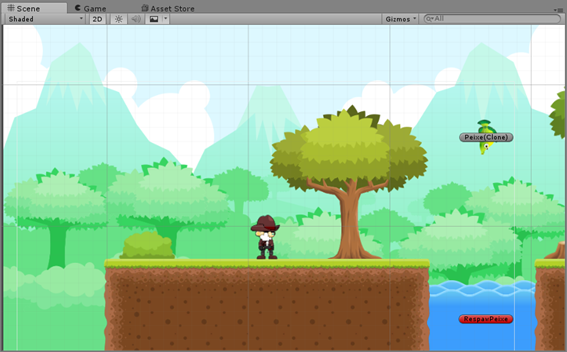
\includegraphics[width=0.7\linewidth]{Imagens/08}
					\legend{Fonte: O autor.}
					\label{fig:08}
				\end{figure}
				
				
			\subsubsection{Game Objects}
				Os \textit{Game Objects} representam quase todos os elementos dentro de uma \textit{scene}, sendo estes uma parte fundamental do projeto. Todos os \textit{Game Objects} de uma \textit{scene} são mostrados na aba \textit{hierarchy}, onde pode-se editá-los e relacioná-los  conforme se faz necessário. \textit{Player}, Camera, Plataforma e os demais objetos listados na aba \textit{hierarchy} são todos \textit{Game Objects}.			
				
				Todos os \textit{Game Object} possuem um componente padrão chamado \textit{Transform}, este é o responsável pode definir sua posição, rotação e escala dentro da \textit{scene}, estes sãos controlados por valores por meio dos eixos x, y e z. Todos os valores presentes neste componente pode ser alterado por meio de \textit{script} ou dentro do próprio \textit{Unity}.
				
			\subsubsection{Components}
				Os \textit{components} são partes fundamentais que compõem os \textit{game objects}, estes são responsáveis por fornecer as características essenciais a cada elemento como sua forma. Através dos \textit{components} se faz possível fornecer uma forma, aplicar leis da física, colisões, efeitos sonoros, efeitos visuais dentre outras ações que são fornecidas pela própria ferramenta \textit{Unity}. Todos os componentes de um \textit{game object} são visualizados em uma aba do \textit{Unity} denominada \textit{Inspector}  (Figura \ref{fig:11}).
				
				\begin{figure}[H]
					\caption{\textit{Components} do \textit{game} \textit{object “Player”}.}
					\centering
					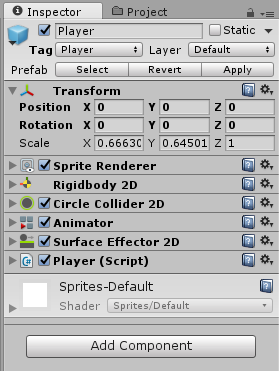
\includegraphics[width=0.5\linewidth]{Imagens/11}
					\legend{Fonte: O autor.}
					\label{fig:11}
				\end{figure}
			
			Na Figura \ref{fig:11} pode-se visualizar todos os componentes que compõe o \textit{game} \textit{object “Player”}, sendo o componente \textit{Transform} responsável por fornecer a sua localização inicial dentro da \textit{scene}, assim como sua rotação e \textit{scala}, o componente \textit{Sprite Renderer} é responsável por conter a \textit{sprite} que é visualizada nas aba \textit{scene}, o \textit{Rigidbody 2d} e o componente responsável por fornecer ao objeto a possibilidade de sofrer ação das leis da física, \textit{Circle Collider 2d} é um colisor, os colisores determinam uma área de colisão, no caso uma circular, que pode ser utilizado para evitar que o objeto possa passar por dentro de outros objetos que possuam outros \textit{colisores}, como as plataformas (Figura \ref*{fig:12}) onde a área retangular na cor verde determina a área de colisão, esse \textit{colisor} é denominado de \textit{Box Collider 2d}, ou pode ser utilizado como um gatilho, onde quando se colidir com a área, convoca-se uma determinada ação, o componente \textit{Animator} responsável por adicionar efeitos animados ao objeto, como o de correr ao movimentar o objeto pela fase, \textit{Surface Effector 2d} adicionar efeitos como fricção entre objetos e suavização de colisões, o \textit{Player} (\textit{script}), os \textit{scripts} são adicionados aos objetos como os outros componentes, podemos assim entender que quando criamos um \textit{script}, criamos um novo componente que pode ser adicionado ao objeto, \textit{Add Component} é responsável caso necessário por adicionar um novo componente ao objeto, quando for adicionar serão demonstradas as possibilidades disponíveis pela ferramenta.
				
				\begin{figure}[H]
					\caption{Plataformas com \textit{Box Collider 2d} da \textit{scene} “fase01”.}
					\centering
					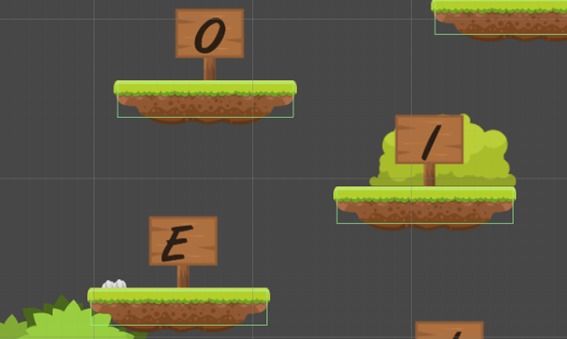
\includegraphics[width=0.6\linewidth]{Imagens/12}
					\legend{Fonte: O autor.}
					\label{fig:12}
				\end{figure}
				No objeto “\textit{Player}” foram utilizado dois \textit{Circle Collider 2d} (Figura \ref{fig:13}) para definir a área de colisão com os outros objetos.
			
				\begin{figure}[H]
					\caption{Objeto \textit{player} na aba \textit{scene} mostrando os colisores.}
					\centering
					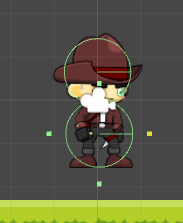
\includegraphics[width=0.4\linewidth]{Imagens/13}
					\legend{Fonte: O autor.}
					\label{fig:13}
				\end{figure}
				
			\subsubsection{Animação}
			Uma animação é criada a partir de uma sequência de imagens (Figura \ref{fig:14}), onde cada imagem deve representar uma parte do movimento, onde o total de imagens correspondem ao movimento completo. Para se criar uma animação no \textit{Unity} se agrupa as imagens que compõem a animação, definindo uma taxa de transição de imagens ideal para que seja fluido aos olhos dos jogadores, e ao executar as imagens serão e exibidas e apagadas conforme a taxa de transição definida.			
				
				\begin{figure}[H]
					\caption{Conjunto de sprites para movimento.}
					\centering
					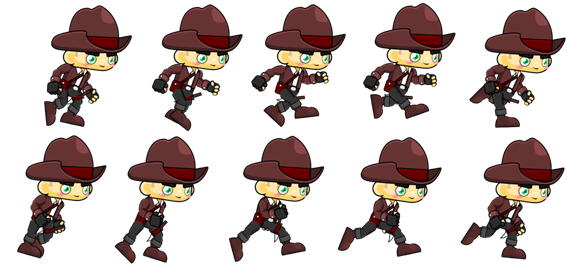
\includegraphics[width=0.6\linewidth]{Imagens/14}
					\legend{Fonte: O autor.}
					\label{fig:14}
				\end{figure}
			
				A velocidade de transição de imagens é configurada pela aba \textit{animation}, assim como a ordem e quais \textit{sprites} pertencem a animação, essa configuração permite que se possa criar uma animação suave com efeitos desejáveis. Pode-se criar mais de uma animação para um \textit{game} \textit{object}, neste caso de faz uso de mecanismo para gerenciar a execução das mesmas.
				
				O gerenciamento das animações, como a troca da animação que contém o efeito de corrida para o efeito de pulo é configurada em uma outra aba, a animator (Figura \ref{fig:16}), onde cada animação possui um estado, esses estados são referenciados no \textit{game object} “\textit{Player}” como \textit{player}\_parado, \textit{player}\_correndo, \textit{player}\_pulando, utiliza-se esses estados através de variáveis podendo fazer a troca de animações no decorrer do jogo.
				Para que se possa executar cada animação em seu devido tempo, após iniciar o jogo, a cada \textit{frame}\footnote{Nos jogos cada \textit{frame} representa um quadro de imagens que é exposto por um determinado tempo}, irá ocorrer um teste sobre as variáveis de estado, sendo assim quando o \textit{player} está se deslocando em linha reta a variável que representa este estado no caso \textit{player}\_correndo muda, recebendo um valor verdadeiro (\textit{true}), então enquanto o valor continuar a ser verdadeiro, ou seja, enquanto o “\textit{Player}” continuar a se movimentar em linha reta a animação do \textit{player} correndo continuará a ser executada, e quando o mesmo parar de se movimentar a variável \textit{player}\_correndo volta ao estado false(\textit{false}), voltando a ser executada a animação padrão, no caso \textit{player} parado.
								
				\begin{figure}[H]
					\caption{Aba \textit{Animator} no \textit{Unity}.}
					\centering
					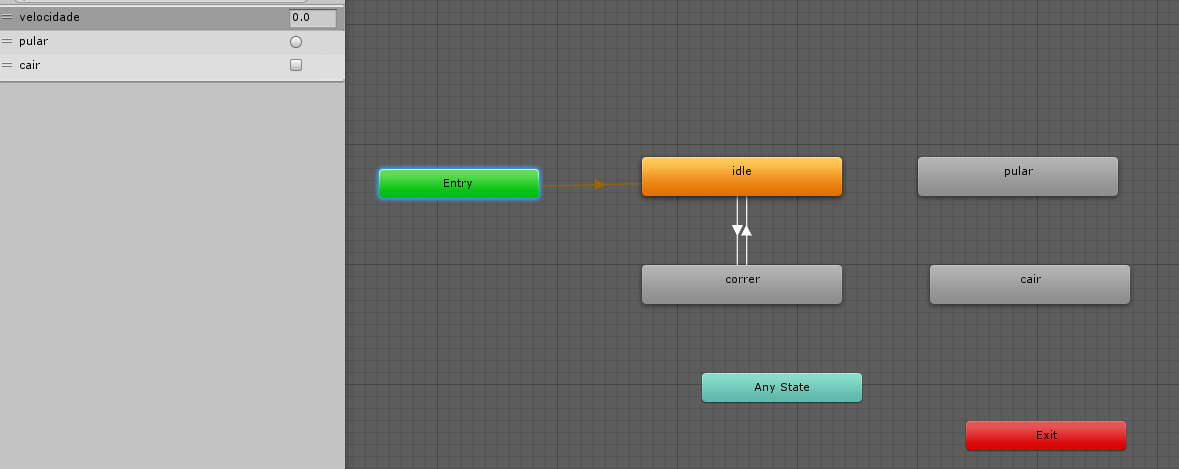
\includegraphics[width=1\linewidth]{Imagens/16}
					\legend{Fonte: O autor.}
					\label{fig:16}
				\end{figure}
				
				
			\subsubsection{Inimigo}
				Normalmente nos \textit{games} os desenvolvedores criam obstáculos a fim de ampliarem a dificuldade e trazerem competitividade. Esses obstáculos podem ser de diversos tipos e formas, podendo possuir ou não inteligência, dependendo exclusivamente da vontade dos desenvolvedores. No \textit{game} apresentado, foram criados alguns inimigos para dificultar o percurso do \textit{player}, um destes inimigos (Figura \ref{fig:17}) possui uma pequena inteligência artificial.
				
				\begin{figure}[H]
					\caption{\textit{Sprite} do inimigo ZumbiM.}
					\centering
					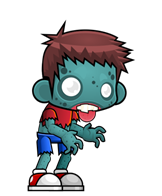
\includegraphics[width=0.4\linewidth]{Imagens/17}
					\legend{Fonte: O autor.}
					\label{fig:17}
				\end{figure}
				
				A forma de criação dos inimigos é semelhante a utilizada para criar o \textit{player}, a diferença básica entre os dois é que o \textit{player} irá ser controlado por uma pessoa, enquanto o inimigo é controlado por um \textit{script} contendo as ações e decisões que este deverá tomar durante a execução do jogo. As animações são criadas da mesma forma que as do \textit{player}, por meio de uma série de \textit{sprites} (Figura \ref{fig:18}), e estados para dar início as animações.
				
				\begin{figure}[H]
					\caption{Conjunto de \textit{sprites} para movimento do Inimigo ZumbiM.}
					\centering
					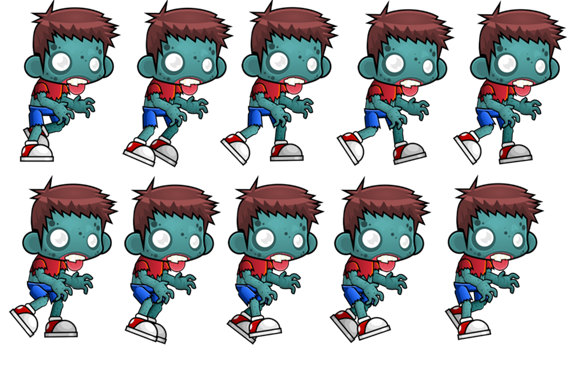
\includegraphics[width=0.6\linewidth]{Imagens/18}
					\legend{Fonte: O autor.}
					\label{fig:18}
				\end{figure}
			
				As ações determinadas ao inimigo são simples, por isso seu \textit{script} não é muito complexo. Uma das funções atribuídas ao inimigo é a de ficar rodeando uma determinada área à espera do \textit{player} para atacá-lo.
				
				
				Uma outra função a ser desempenhada pelo inimigo é a de atacar o \textit{player}, quando o mesmo se infiltrar na área que o inimigo reside, então este deve atacá-lo, caso haja êxito será subtraído um ponto do HP (Vidas) do player, em sequência este será empurrado no sentido contrário ao inimigo. Esse ataque ocorre quando a uma colisão é detectada entre os colisores do \textit{player} e do inimigo, funcionando como gatilhos para as funções.
							
				
			\subsubsection{Efeitos Sonoros}
				Os efeitos sonoros são adicionados por meio de um ou mais \textit{components}, o componente amplamente utilizado no projeto para se adicionar sons é o \textit{Audio Source}, por meio deste componente podemos vincular a um \textit{game object} um arquivo de áudio, o componente fornece a possibilidade definir quando se este áudio deve ser executado ao iniciar o jogo, se deve ser repetido, volume entres outras opções disponíveis. Por meio de \textit{script} pode-se configurar o momento que se deve executar o áudio.
				
				Outro \textit{component} que tem por objetivo a criação de efeitos sonoros é o \textit{Audio Listener}, este tem a função de ser o “ouvido” do jogador dentro do jogo, assim o \textit{player} pode ouvir todos os sons dentro do \textit{game}. Este componente é adicionado ao \textit{Main Camera} que faz o papel dos “olhos” aos jogadores.		
	
	\subsection{Definições de Final de Jogo}
		As definições de final de jogo é uma parte importante do planejamento, nela se esclarece o que deve acontecer quando o jogo deve terminar. Na implementação se tem duas opções de final de jogo, sendo uma a tela de \textit{game over}, esta tela é responsável por avisar ao \textit{player} que o mesmo falhou no seu objetivo de chegar ao final, e que ele deve recomeçar o trajeto, a regra para que seja chamada a tela de \textit{game over} é a de que o personagem perca todas as suas vidas, ao inciar o jogo o mesmo começa com 5 vidas que podem ser incrementadas ou decrementadas conforme o avanço, quando estas chegarem a 0 a função responsável deve efetuar a chamada de tela de \textit{game over}.
		
		O personagem pode incrementar seus pontos de vida conforme avança na respectiva fase, isto irá ocorrer quando o mesmo colidir com um objeto especial denominado “1UP” (Figura \ref*{fig:22}). O decremento de pontos de vida ocorre em dois momentos distintos, sendo o primeiro quando o mesmo colidir com um inimigo que o ataca, onde cada ataque decrementa um ponto de vida ou quando o mesmo cai na água, onde é decrementada um ponto de vida e o mesmo retorna uma parte do que avançou.
		
		\begin{figure}[H]
			\caption{Item “1UP”}
			\centering
			
\includegraphics[width=0.3\linewidth]{Imagens/22}
			\legend{Fonte: O autor.}
			\label{fig:22}
		\end{figure}		
		
		O sistema de avanço de fase utilizado no projeto é simples, onde para conseguir avançar o \textit{player} deve chegar no castelo de pedra (Figura \ref*{fig:23}) no final da fase, onde este serve como gatilho para iniciar o desfaio da fase. 
		
		\begin{figure}[H]
			\caption{Castelo de pedra no final da fase}
			\centering
			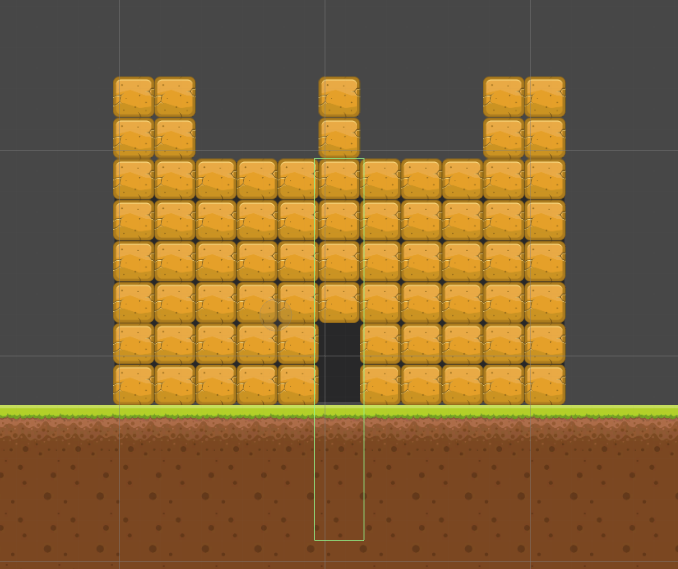
\includegraphics[width=0.7\linewidth]{Imagens/23}
			\legend{Fonte: O autor.}			
			\label{fig:23}
		\end{figure}
	
		Um outro ponto a ser observado e de grande importância são os desafios, estes são imposto afim de bloquear a passagem do \textit{player} para a próxima fase, sendo necessário completa-lo para que inicie a próxima fase. O primeiro desafio imposto ao jogador é um jogo da memória (Figura \ref*{fig:25}) que possui 5 pares a serem encontrados, quando o jogador encontrar todos a 2 fase se inicia.
		
		\begin{figure}[H]
			\caption{Primeiro desafio, jogo da memoria}
			\centering
			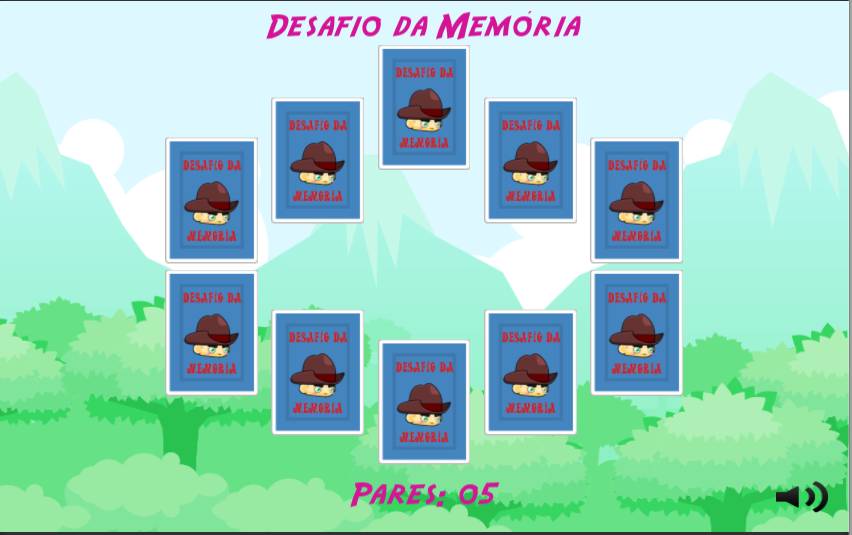
\includegraphics[width=0.7\linewidth]{Imagens/25}
			\legend{Fonte: O autor.}
			\label{fig:25}
		\end{figure}		
		
		Quando se termina um desafio a próxima fase é chamada, assim o mesmo processo irá se repetir sendo o próximo desafio de grau diferente do anterior. Quando o \textit{player} passar pelo o desafio final e logo após encontrar a “Aventureira”\footnote{Personagem parceira do \textit{player} que se encontra no final do jogo o esperando para novas aventuras} o jogo finaliza na tela de sucesso (Figura \ref*{fig:24}).
		\begin{figure}[H]
			\caption{Tela de sucesso final}
			\centering
			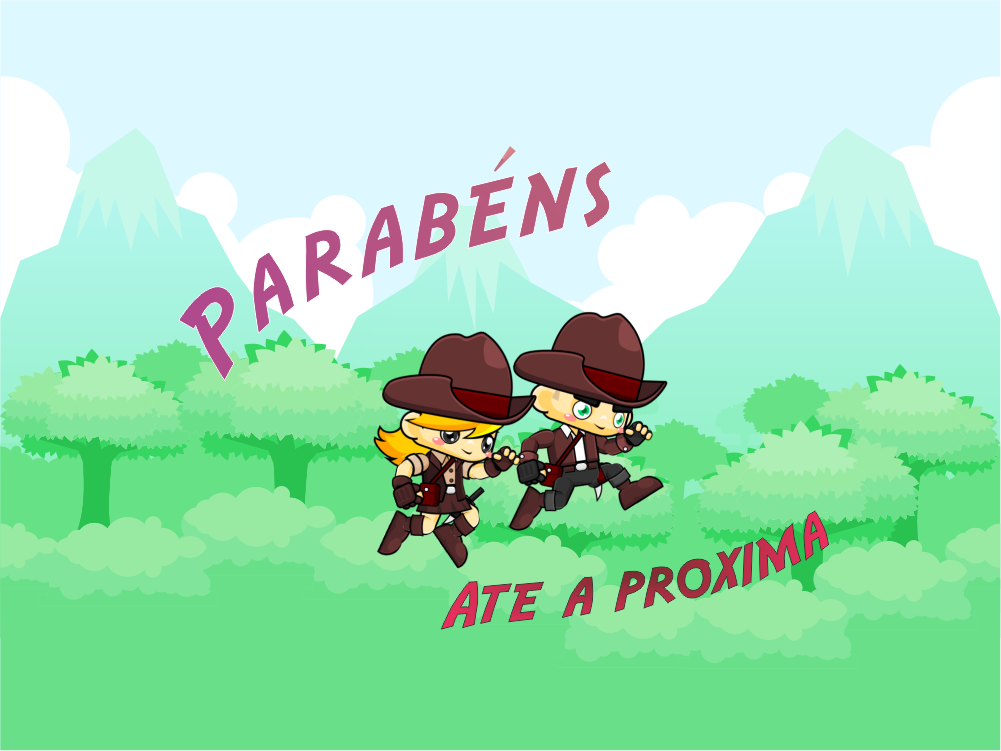
\includegraphics[width=0.7\linewidth]{Imagens/24}
			\legend{Fonte: O autor.}
			\label{fig:24}
		\end{figure}
		
	
\section{Avaliação}

	Os testes são uma parte fundamental de qualquer projeto, sem estes se torna impossível afirmar que a ferramenta desenvolvida cumpre com o prometido. A utilização dos testes no desenvolvimento de \textit{softwares} é uma parte muito importante, e que recebe um cuidado especial. Geralmente nas equipes de desenvolvimento se encarrega um profissional somente para essa parte, assim maximizando a possibilidade de encontrar erros a serem corrigidos. Os testes servem de base para melhorias, através destes pode-se incluir funcionalidades ou remove-las, se as mesmas não agregarem valor ao produto. Os testes propostos neste trabalho têm como finalidade verificar a sua eficácia, erros e possíveis melhorias a serem propostas pelos usuários.
	
	\subsection{Participantes}
	
	O projeto desenvolvido neste trabalho foi disponibilizado para alunos da Escola Municipal Santa Catarina da Rede Pública Municipal de Ensino da cidade de Ipiranga do Piauí para ser testado e avaliado, além disso o mesmo foi disponibilizado para professores e diretoria para fins de conhecimento. A diretoria e professores ficaram responsáveis por convidarem os alunos para efetuarem os testes, onde estes foram divididos em dois grupos de controle, sendo o primeiro grupo, os de alunos que não possuem distúrbio de atenção e hiperatividade ou qualquer outra alteração, o segundo e composto por alguns alunos que possuem diagnóstico de distúrbio de TDAH, entre eles alguns possuem comorbidades\footnote{Ocorrência de mais de um problema ao mesmo tempo}, e outros que se tem desconfiança por apresentarem os sintomas em sala de aula.
	
	Durante os testes, foram observadas 16 crianças, com idades variando de 6 a 10 anos, e que frequentam do 1ª ao 5ª ano do ensino fundamental. As crianças foram divididas em dois grupos, onde se tem 8 crianças em cada, de forma proporcional a suas idades e ano que frequentam. 
	
	\subsection{Metodologia de Teste}
		Os testes ocorreram de forma individual, sendo assim foi disponibilizado ao aluno um computador com o jogo em execução, além de um local com pouca interferência de terceiros, no mesmo permaneceram somente o aluno, pesquisador e professor responsável pelo local. O teste de cada aluno foi dividido em duas partes, sendo:
		
			\begin{itemize}
				\item Ocorreu de forma observativa, onde o pesquisador analisou e documentou, através de um questionário, as alterações ocorridas enquanto o aluno testava a ferramenta, como nível de concentração, entendimento, se houve dificuldades na execução, o tempo que levou para completar as atividades;
				
				\item Em forma de entrevista entrevista, foram feitos algumas perguntas para cada aluno após o fim da execução do teste, para que assim os mesmos avaliassem a ferramenta, apontarem onde podem haver melhorias, quais os pontos negativos, que chamou mais a atenção, o que gostariam de adicionar.
			\end{itemize}
		
			Durante a análise foi atribuída um valor que pode variar de 0 (pior caso) a 5 (melhor caso) aos seguintes requisitos observados: 
			\begin{itemize}
				\item Nível de concentração durante os testes -  este ponto é o principal a ser observado pelo fato que o maior problema enfrentado por portadores de TDAH é a dificuldade de manter concentração em atividades que possam a entediantes, este requisito demostra o quanto o aluno está empenhado em desenvolver a atividade, se houve distrações;
				
				\item Nível de dificuldade - neste ponto é analisado a dificuldade enfrentada ao desempenhar as atividades, onde é atribuída uma nota para cada fase testada, e após o fim é registrado uma média geral de dificuldade enfrentada no jogo. As notas em cada fase servem de base para saber onde encontraram problemas desnecessários, o que não conseguiram solucionar, para que assim possa ser feita correções;
				
				\item Avaliação dos alunos - Na entrevista os alunos podem dar uma nota para a ferramenta, assim se torna possível analisar o quanto gostaram da experiencia com jogos educativos;
				
				\item Tempo gasto - A análise do tempo gasto serve para medir o desempenho de cada aluno, ja que ainda não se tem implementado um sistema de \textit{score}\footnote{Sistema para medir desempenho e pontuação};
			\end{itemize}
		
		Em sala de aula, os participantes foram observados enquanto faziam suas atividades escolares, durante essa observação foi analisado seu comportamento e nível de concentração enquanto desempenhavam as atividades em sala de aula. Ao final da análise de cada aluno que participou dos testes, estes receberam uma nota referente ao nível de concentração e atenção nas atividades desempenhadas. E de grande importância a análise do comportamento de cada participante em outras atividades que envolvam o ensino e aprendizagem, só assim pode-se verificar se a ferramenta está obtendo resultados positivos ou negativos.
	\subsection{Resultados}
			 
	Para se medir o desempenho do Grupo 2 composto por crianças com TDAH e comorbidades, os dados de todos os participantes foram somados para se obter uma média geral de cada requisito, o mesmo aconteceu com os resultados do Grupo 1 composto por crianças sem TDAH ou outros problemas que possam influenciar. Os resultados dos testes podem ser visualizados por meio da Tabela \ref*{tabela1}.
		
		\begin{table}[H]
			\centering
			\caption{Média dos resultados obtidos nos testes.}
			\label{tabela1}
			\begin{tabular}{|l|l|l|}
				\hline
				\textbf{Requisitos}                                                             & \textbf{Grupo 1} & \textbf{Grupo 2} \\ \hline
				Nível de Concentração                                                           & 4,5625           & 4,4375           \\ \hline
				Dificuldade enfrentada                                                          & 3,1875           & 3,3125           \\ \hline
				Tempo Gasto                                                                     & 16 minutos       & 20 minutos       \\ \hline
				Nota dada a ferramenta                                                          & 4,25             & 4,375            \\ \hline
				\begin{tabular}[c]{@{}l@{}}Quantidade de alunos que \\completaram a atividade\end{tabular} & 8                & 8                \\ \hline
			\end{tabular}		
			\legend{Fonte: O autor.}
		\end{table}
		
		Com base nos resultados apresentados é possível perceber que o Grupo 2, apesar de possuir notas inferiores nos requisitos, a diferença não é tão acentuada. O principal requisito analisado nos testes é o de concentração que representa a atenção e comportamento, pois está estritamente atrelado aos problemas enfrentados pelos portadores de TDAH. Apesar da nota do Grupo 2 no requisito concentração ser menor que a do Grupo 1, percebe-se mesmo assim um alto desempenho.
	
		Para verificar o desempenho dos participantes em outras atividades se utilizou o mesmo tipo de análise observativa, assim tornou-se possível obter uma média do nível de concentração dos dois grupos, como as atividades desempenhadas em salas de aula possui metodologias diferenciadas das utilizadas no jogo, se descartou os demais requisitos. Os resultados das análises podem ser vistos na Tabela \ref*{tabela2}.
	
		
		\begin{table}[H]
			\centering
			\caption{Resultado do nível de concentração dos alunos nas atividades ocorridas em sala de aula}
			\label{tabela2}
			\begin{tabular}{|l|l|l|}
				\hline
				Requisito             & Grupo 1 & Grupo 2 \\ \hline
				Nível de Concentração & 3,4375  & 2,875   \\ \hline
			\end{tabular}
			\legend{Fonte: O autor.}
		\end{table}
		
		Quando comparado os resultados entre as atividades, é perceptível o aumento da concentração dos alunos quando estão utilizando a ferramenta, principalmente os alunos do Grupo 2 que possuem TDAH, neste percebe-se um amento de 31,5\% do nível de concentração em relação as outras atividades executadas em sala de aula.
		
		\subsection{Considerações Finais}
		
		Apesar dos testes ainda serem insuficientes para se ter resultados concretos, os dados obtidos já se mostram promissores, principalmente quando comparados os níveis de concentração obtidos durante os testes, atestando que os alunos aprovam a ideia de utilizar o \textit{game} desenvolvido como ferramenta de aprendizagem. Um dos maiores problemas enfrentados pelos portadores de TDAH na aprendizagem sem dúvida é a dificuldade de manter a atenção, pois estes alunos perdem o foco com muita facilidade. O fato dos alunos conseguirem uma nota muito próxima a de alunos sem TDAH, comprova que quando utilizado a ferramenta adequada os portadores de TDAH podem ter o mesmo nível de concentração, e consequentemente, o mesmo desempenho de pessoas sem o transtorno.
		
	
% ---

% Conclusão
% ---
\chapter{Conclusão}

	Apesar dos portadores de TDAH enfrentarem obstáculos em seu processo educacional, estes podem ser superados utilizando-se ferramentas adequadas. A utilização de um \textit{game} como ferramenta auxiliar de ensino se mostrou muito promissora, onde os portadores apresentaram um nível de concentração quase igual a de crianças normais, podendo favorecer o processo de aprendizagem para alunos que possuam problemas de concentração e déficit de atenção.
	
	O jogo em si não deve servir como professor para alunos com TDAH, mais poderá servir como ferramenta para professores que ensinam alunos com o transtorno, estes poderão utilizar de forma dinâmica tais jogos para ensinarem estes alunos. Um cuidado deve ser tomado com este tipo de ferramenta, pois se utilizada de maneira inadequada, sem acompanhamento de educadores capacitados, esta que deveria ajudar pode acabar atrapalhando o processo de ensino, pois o aluno poderá sofrer de desvios em seu aprendizado, por isso a necessidade de alguém para guia-lo.	
	
	Apesar da ferramenta apresentar resultados promissores, ainda a muito trabalho a ser desenvolvido, fazendo-se necessário mais testes para avaliar quais pontos devem ser modificados, o que deve ser adicionado e onde devem ser colocados. E perceptível a necessidade haver uma integração e troca de conhecimentos entre desenvolvedores e profissionais da área da educação, principalmente os de educação especial, só assim é possível encaixar metodologias de ensino empregadas em salas de aulas que podem colaborar na qualidade da ferramenta.
	
	Por tudo que foi apresentado, é possível perceber a necessidade de adicionar mais atividades dinâmicas como os jogos nos processos de ensino a crianças com TDAH. A utilização do \textit{Adventures of Learning} para melhorar o processo de aprendizagem se mostrou eficaz no que se propôs a fazer, prendendo a atenção do usuário na ferramenta lhe fornecendo ensino e divertimento.
	
	Para trabalhos futuros, pretende-se aperfeiçoar o que já foi desenvolvido, realizando-se mais testes em maior tempo para se obter resultados concretos acerca da ferramenta, trazer novas fases e desafios com novos conteúdos a serem explorados. Pretende-se trabalhar em conjunto a educadores, trazendo ao \textit{game} novas ideias e metodologias a serem aplicadas para melhorar o processo de ensino.
	Realizar a distribuição para outras plataformas, possibilitando que educadores possam utilizar a ferramenta em outros equipamentos para melhor aplicabilidade.
	
% ----------------------------------------------------------
% ELEMENTOS PÓS-TEXTUAIS
% ----------------------------------------------------------
\postextual


% ----------------------------------------------------------
% Referências bibliográficas
% ----------------------------------------------------------
\bibliography{references} %% REFERENCIA AO ARQUIVO abntex2-modelo-references.bib

% ----------------------------------------------------------
% Glossário
% ----------------------------------------------------------
%
% Consulte o manual da classe abntex2 para orientações sobre o glossário.
%
%\glossary
% ----------------------------------------------------------
% Apêndices
% ----------------------------------------------------------
% ---
% Inicia os apêndices
% ---
\begin{apendicesenv}
% Imprime uma página indicando o início dos apêndices
\partapendices
% ----------------------------------------------------------
\chapter{Termo de Autorização}
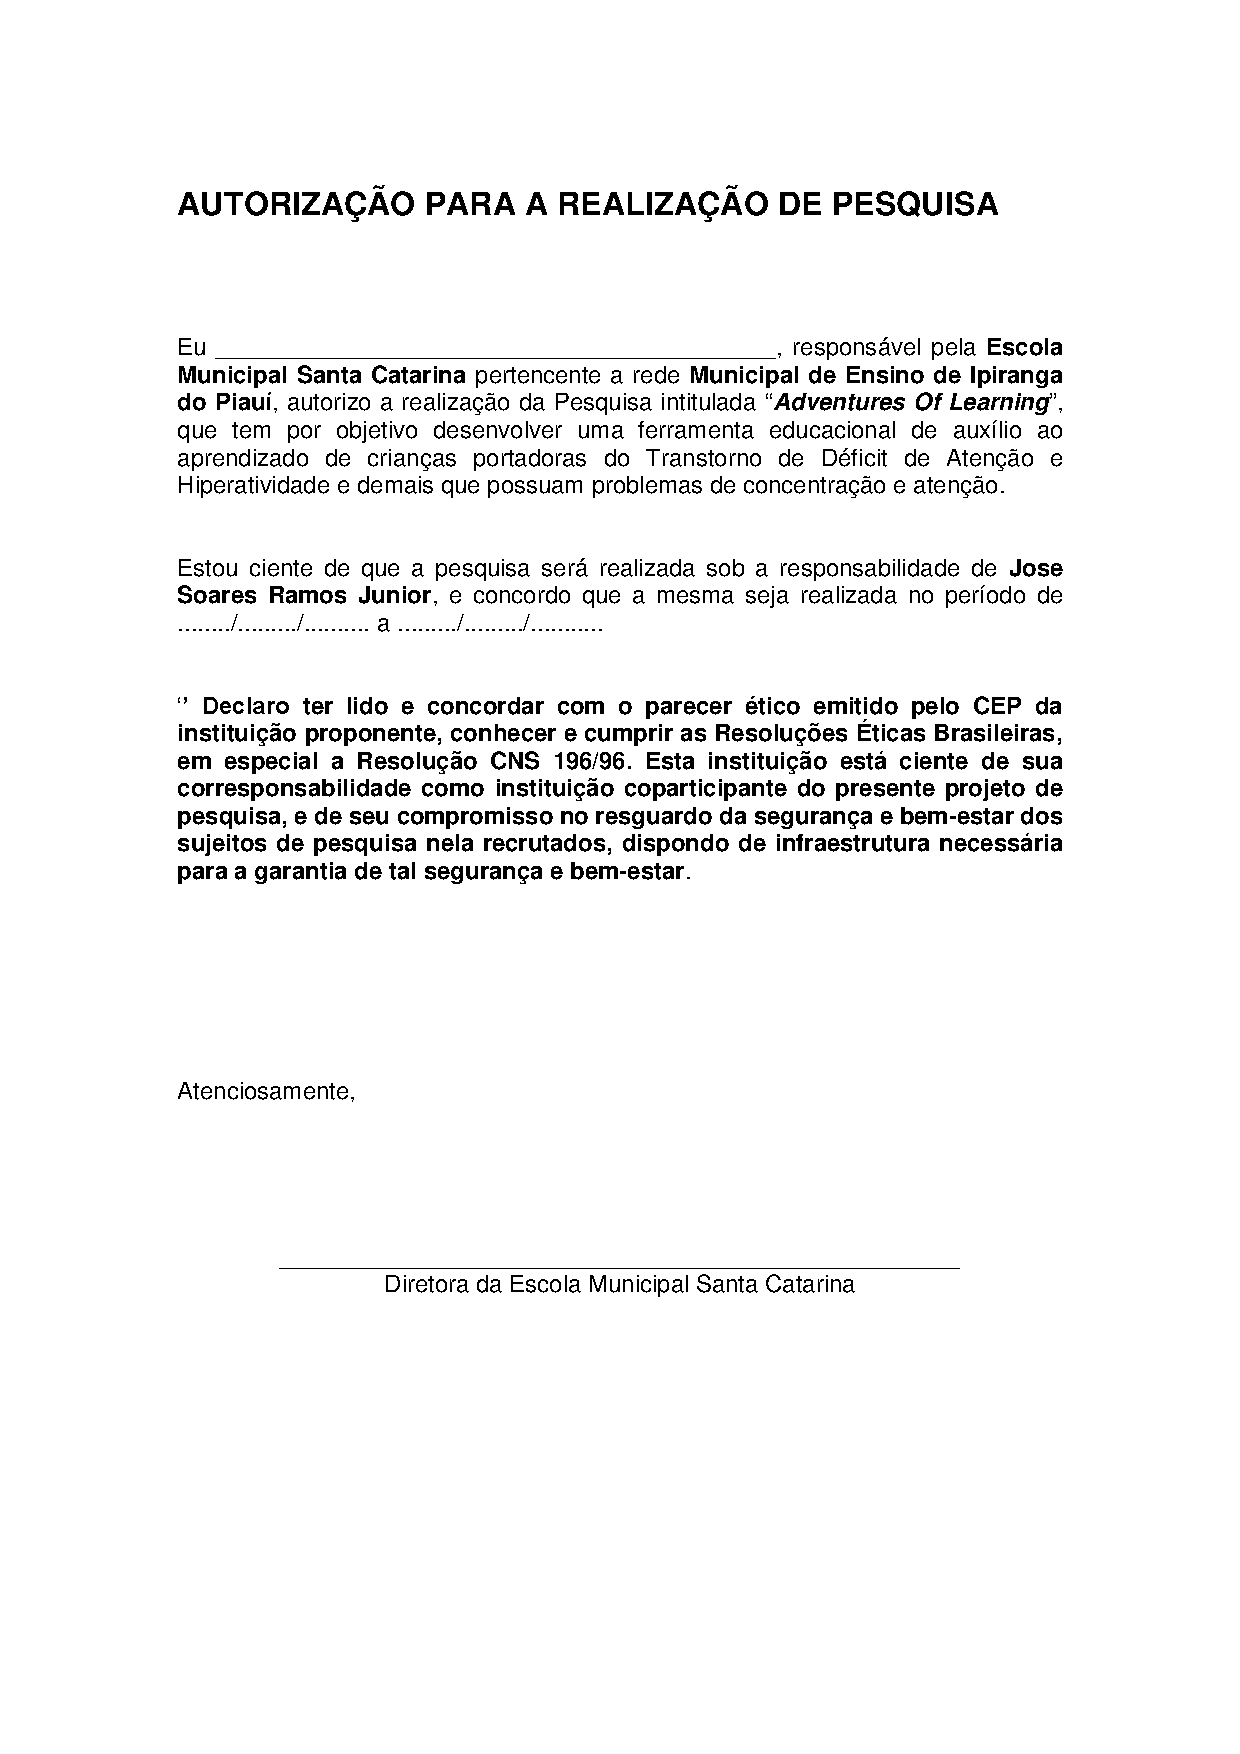
\includepdf[pages=1]{autorizacao.pdf}
\chapter{Termo de Consentimento}
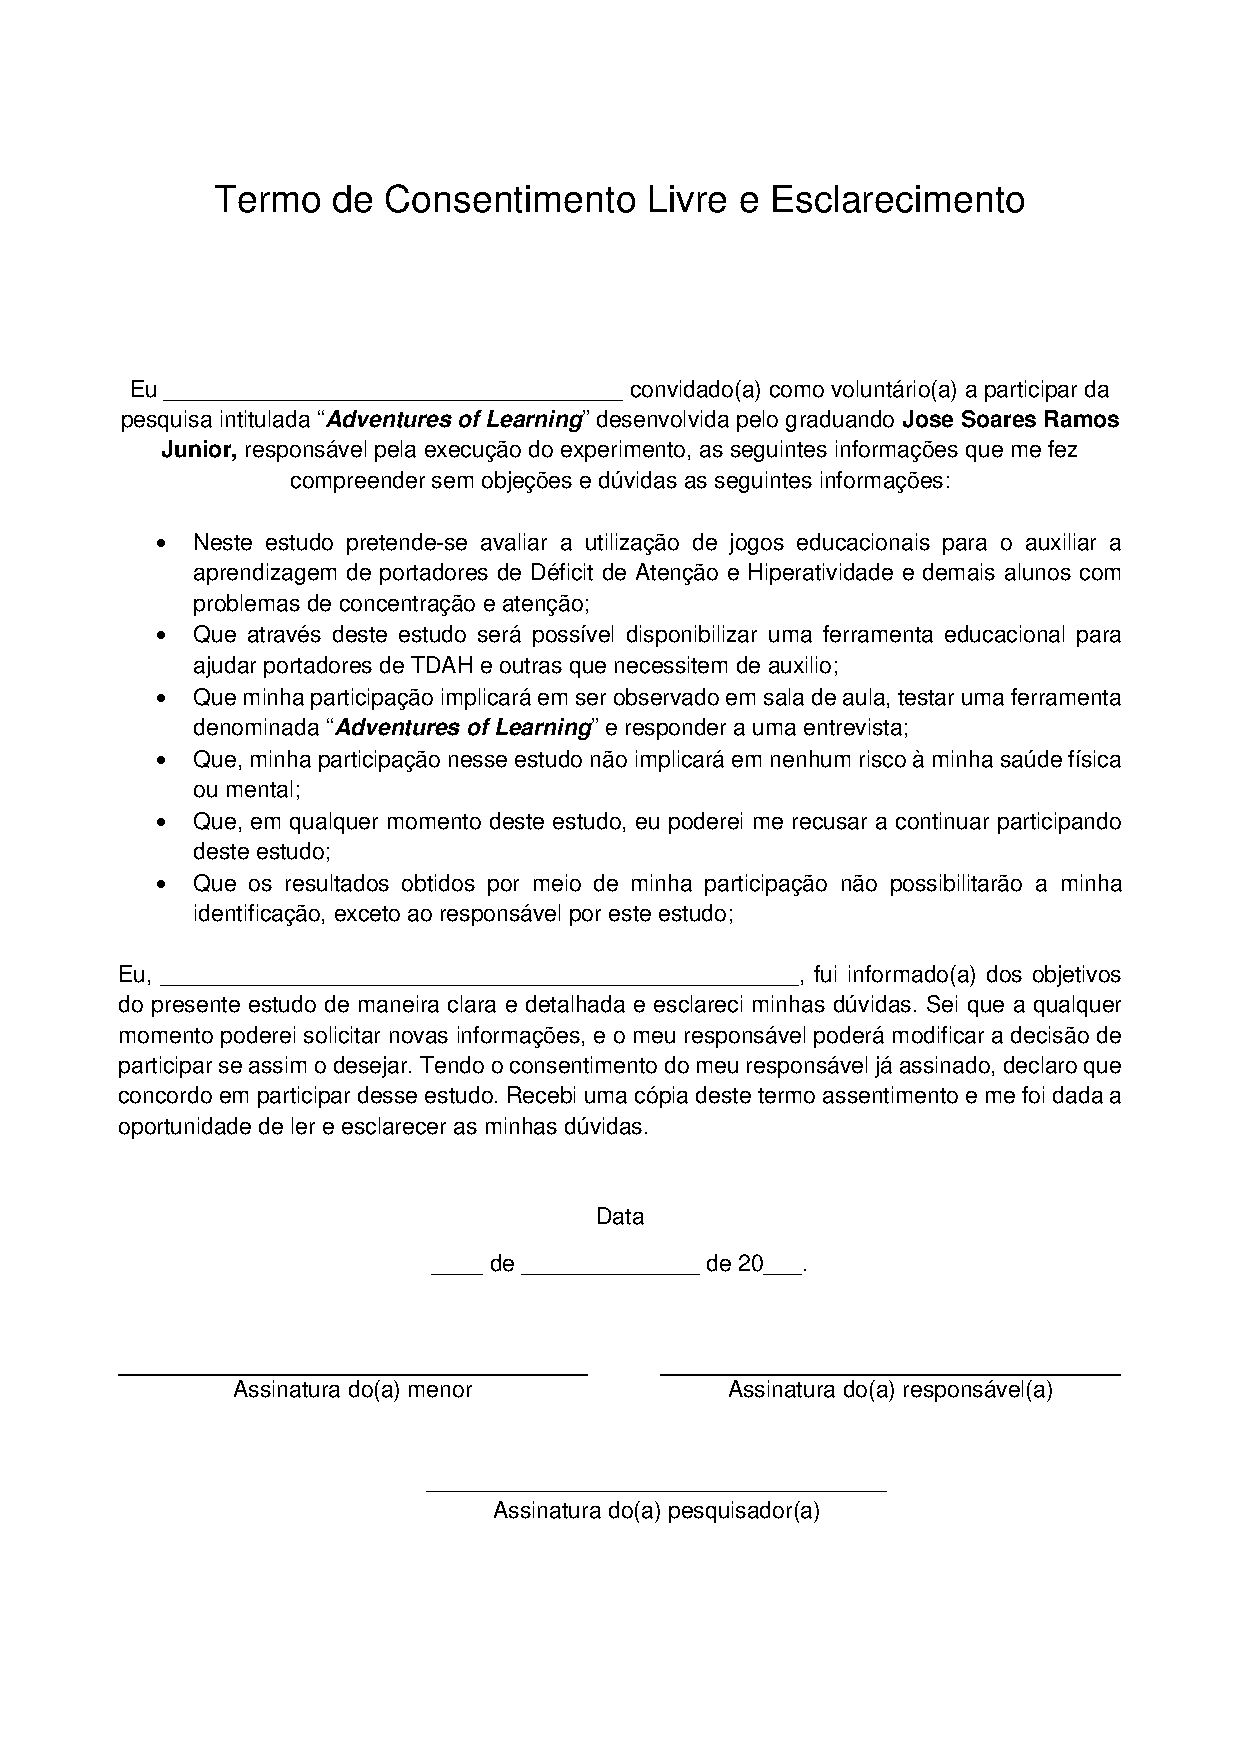
\includepdf[pages=1]{termo.pdf}
\chapter{Ficha de Avaliação de Comportamento Geral}
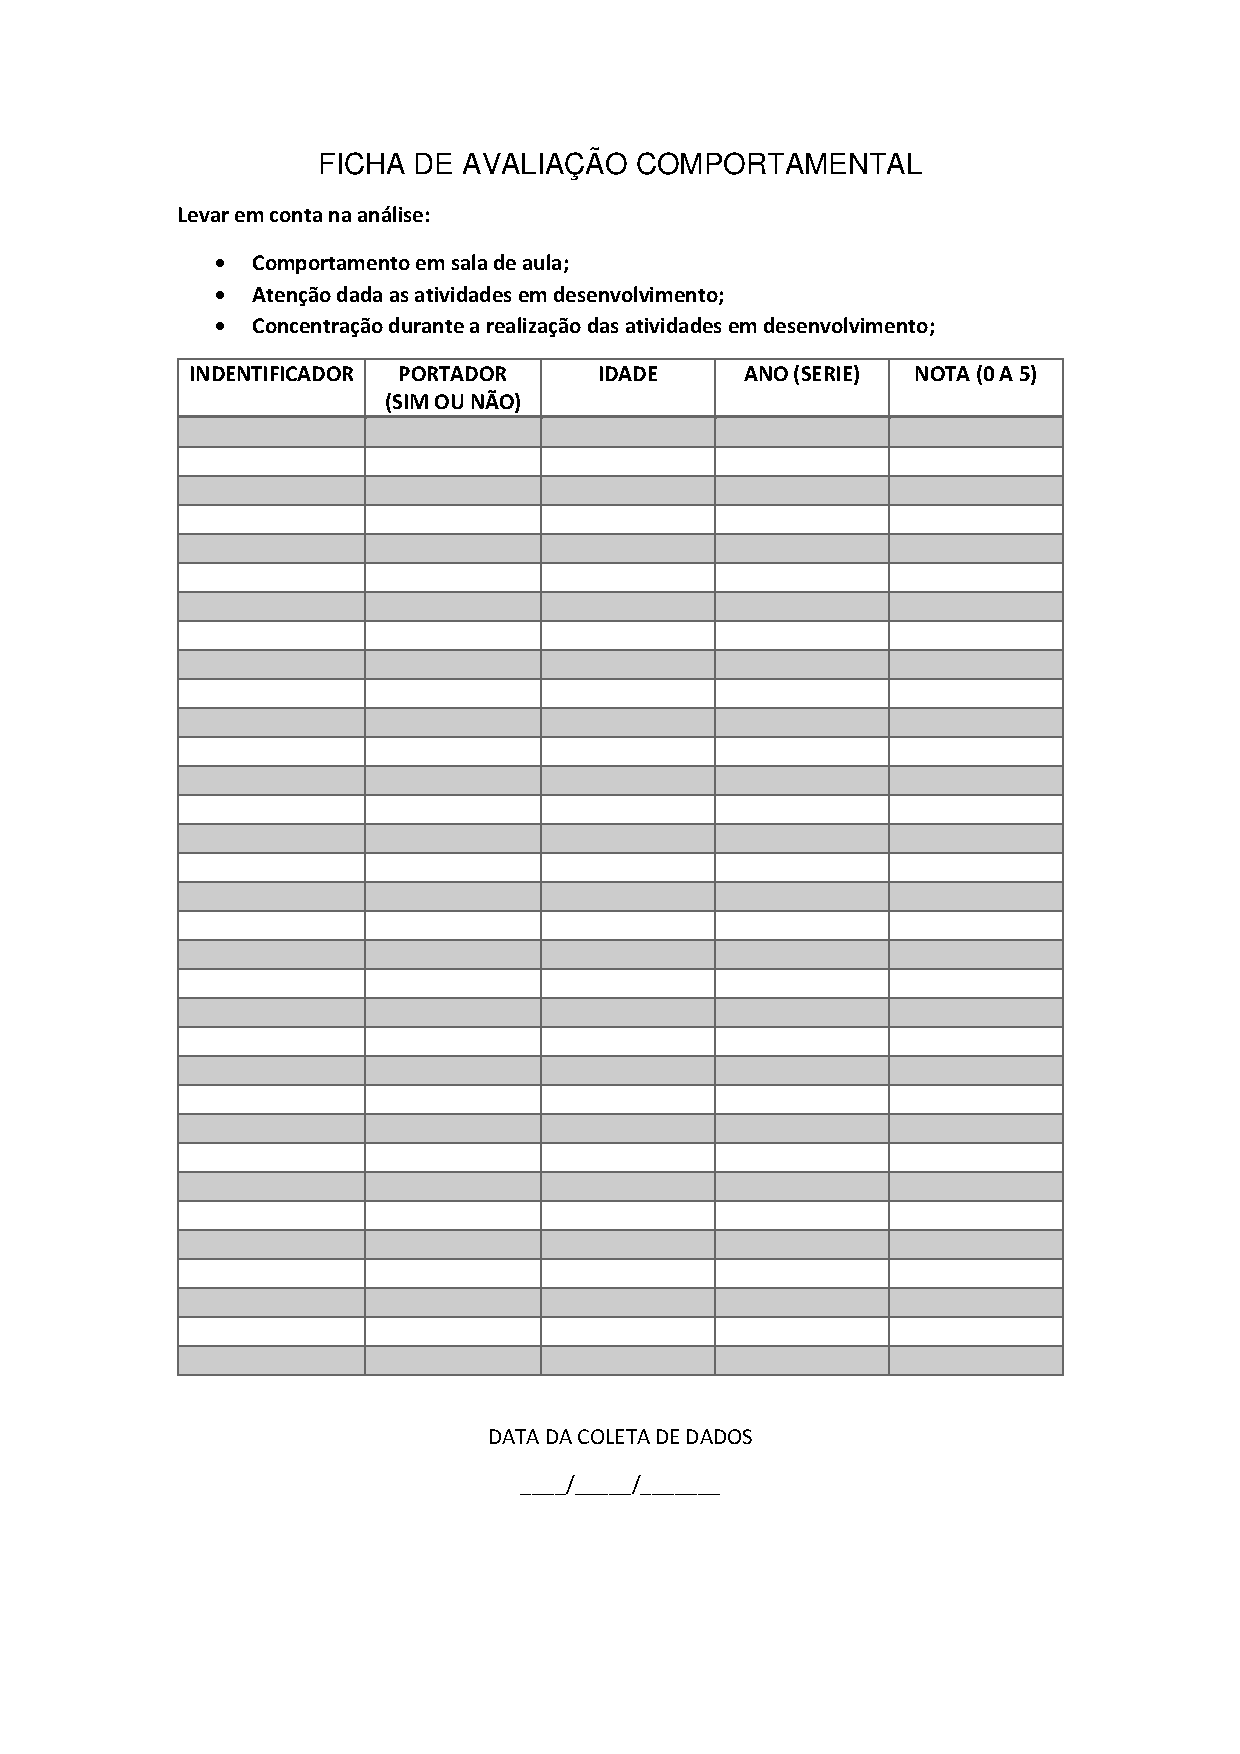
\includepdf[pages=1]{fichageral.pdf}
\chapter{Ficha de Avaliação Individual}
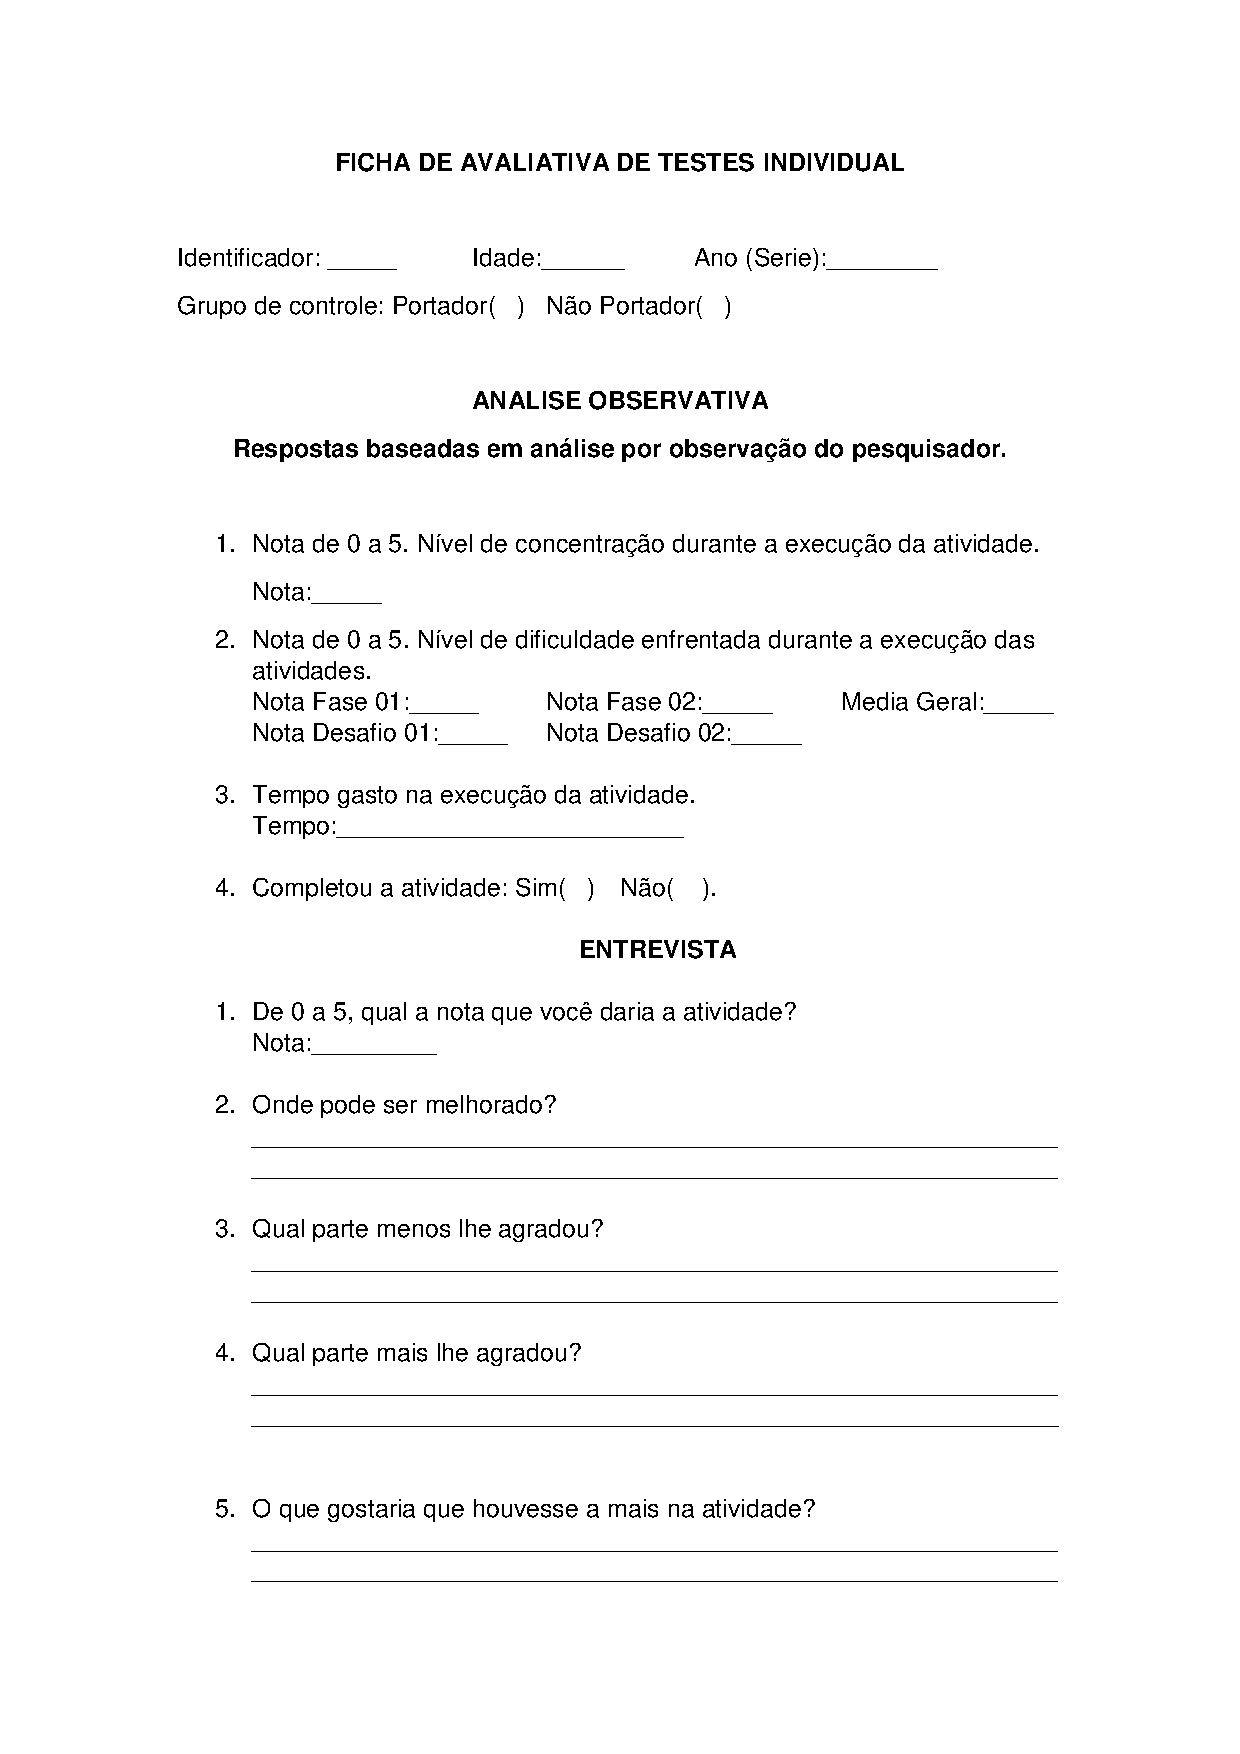
\includepdf[pages=1]{fichaindividual.pdf}
% ----------------------------------------------------------
\end{apendicesenv}
% ---
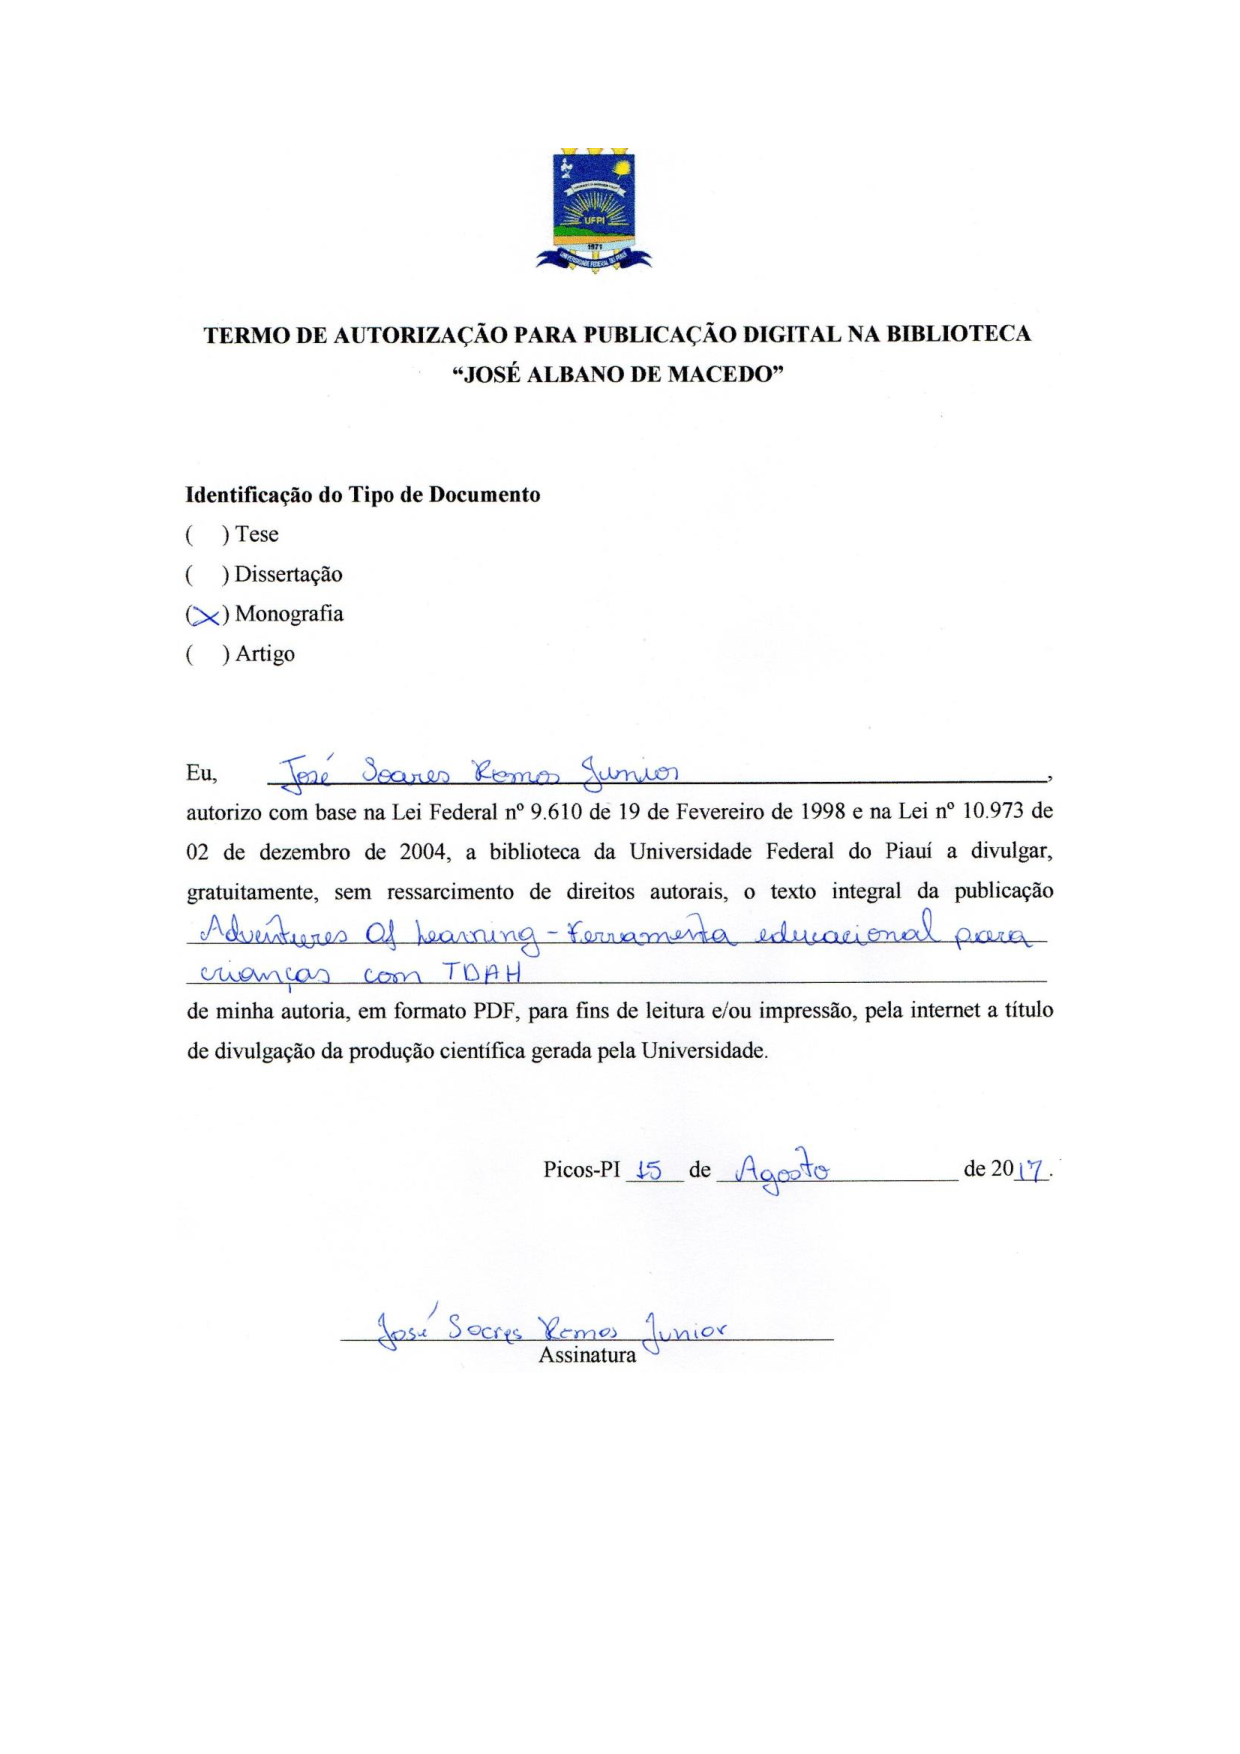
\includepdf[pages=1]{termo-publicacao.pdf}	

\end{document}
